%%
%% This is file `mcmthesis-demo.tex',
%% generated with the docstrip utility.
%%
%% The original source files were:
%%
%% mcmthesis.dtx  (with options: `demo')
%%
%% -----------------------------------
%%
%% This is a generated file.
%%
%% Copyright (C)
%%     2010 -- 2015 by Zhaoli
%%     2014 -- 2016 by Liam 
%%     2017 -- 2019 by Xuehan
%%
%% This work may be distributed and/or modified under the
%% conditions of the LaTeX Project Public License, either version 1.3
%% of this license or (at your option) any later version.
%%
%% This work has the LPPL maintenance status `maintained'.
%%
%% The Current Maintainer of this work is Xuehan.
%%
\documentclass{mcmthesis}
\mcmsetup{CTeX = false,   % 使用 CTeX 套装时,设置为 true
        tcn = 2100462, problem = E,
        sheet = true, titleinsheet = true, keywordsinsheet = true,
        titlepage = false}
\usepackage{palatino}
\usepackage{mwe}
\usepackage{graphicx}
\usepackage{subcaption}
\usepackage{float}
\usepackage{multirow}
\usepackage{indentfirst}
\usepackage{gensymb}
\usepackage[ruled,lined,commentsnumbered]{algorithm2e}
\usepackage{diagbox}
\usepackage{url}
\usepackage{cite}
\usepackage{hyperref}
\documentclass{ctexart}
\usepackage[ruled,vlined]{algorithm2e}
\usepackage{algpseudocode}  
\usepackage{amsmath}  
\bibliographystyle{ieeetr}
\usepackage{geometry}
\def\UrlBreaks{\do\A\do\B\do\C\do\D\do\E\do\F\do\G\do\H\do\I\do\J \do\K\do\L\do\M\do\N\do\O\do\P\do\Q\do\R\do\S\do\T\do\U\do\V \do\W\do\X\do\Y\do\Z\do\[\do\\\do\]\do\^\do\_\do\`\do\a\do\b \do\c\do\d\do\e\do\f\do\g\do\h\do\i\do\j\do\k\do\l\do\m\do\n \do\o\do\p\do\q\do\r\do\s\do\t\do\u\do\v\do\w\do\x\do\y\do\z \do\.\do\@\do\\\do\/\do\!\do\_\do\|\do\;\do\>\do\]\do\)\do\, \do\?\do\'\do+\do\=\do\#}
\geometry{left=2cm,right=2cm,top=2cm,bottom=2cm} %%页边距,若对左右边距进行修改,请保证左右边距一样,并且将mcmthesis.cls第81行对应的margin参数设置为相同数值
\begin{document}
\linespread{0.6} %%行间距
\setlength{\parskip}{0.5\baselineskip} %%段间距
\title{SEPEG Model: Betake Food System To Sustainability And Equity}

\date{\today}
\begin{abstract}
 	 
Generally speaking, the existing food system plays an indispensable role in the whole process of worldwide food production, circulation and distribution. Nevertheless, it is undeniable that the existing food system has already shown its defects and vulnerability reflected from some recent news in the global scale, which mainly attributes to the current preference of profitability and efficiency. Aiming to cover the shortage and optimize the food system, our team proceed as follows:
 	
Firstly, we dissect the data downloaded from FAO's official website and scope 6 typical Asian countries in our consideration. To evaluate the food system more comprehensively, we carefully select \textbf{10 indexes} subordinated to \textbf{5 indicators}, namely \textbf{sustainability}, \textbf{equity}, \textbf{profitability}, \textbf{efficiency} and \textbf{globalization factor}. Intended to pursue equity and sustainability, we then obtain the combined weights of 5 indicators through both objective evaluation by \textbf{EWM} and subjective revision by \textbf{AHP}. Through \textbf{Roulette Wheel Selection} and further process of the indexes, we launch the \textbf{Sustainability-Equity-Profitability-Efficiency-Globalization Model} (\textbf{SEPEG Model}). Through time series prediction and combining with specific cases, we calculate the time necessarily required to implement the new food system.

To further probe the features of the optimized system, we continue to explore the disparities between them in the next part. We sum up the benefits and costs comparing the food system after being optimized by SEPEG Model with before. Without losing generality, we choose Japan and Indonesia as verified objects of our model, for Japan represents developed country and the other stands for the developing. By comparative analysis of the indexes, some differences between developed countries and the developing ones are concluded. At last, we explore when these changes would happen according to different indexes, which are classified into four types.
 	  
Then, we continue to research the feasibility of the \textbf{Zero Hunger} goal mapped out by UN five years ago. Based on SEPEG Model, combined with \textbf{ARIMA} and \textbf{Grey Model}, we give the predictions of Hunger Index and Food Insecurity Index of Indonesia in 2030, one typical underdeveloped and populous country. Unfortunately, the grand vision may not be accomplished based on the current situation before the scheduled deadline.
 	  
At last, we validate the \textbf{extensibility and adaptability} of SEPEG Model by selecting other regions and nations such as east and southeast Asia and the Republic of Korea. Subsequently, through sensitivity analysis, we find out the uncertainty of SEPEG Model is weak and the model has the characteristic of robustness. Finally, integrated with strengths and weaknesses, we make a comprehensive assessment of SEPEG model.
\\
	\begin{keywords}
	\textbf{Food System, Entropy Weight Method, Analytic Hierarchy Process, Roulette Whell Selection, ARIMA, Grey Model}
	\end{keywords}
\end{abstract}

\maketitle
\tableofcontents

\newpage
\section{Introduction}

\subsection{Background}

In the past year, the pandemic of COVID-19 has wreaked havoc on the global food system, even in places it previously revolves well. This indicates the existing system is still vulnerable and labile, which is
attributed to the current preference for profits and efficiency to some degree. Those producers and distributers who have already occupied massive share of global market give priority to operating the system efficiently and making revenues.

However, the statistics estimated before the epidemic is already staggering and horrendous. 8.9$\%$ of the world's population, nearly 821 million people, are still suffered from hunger. What's worse, the current system has already caused irreversible damage to the environment, which includes 29$\%$ of greenhouse emissions, 80$\%$ of diversity loss and 80$\%$ of deforestation\cite{statistics}. This all suggests that the food system, the networks needed to produce, process and distribute, fails to meet social demands. Further improvements to the food system and its ability to realize sustainable development will therefore be the key. In such case, it's of vital significance to reexamine the current condition thoroughly to further optimize it.

\subsection{Problem Restatement}
 To serve the interests of mankind, ICM Committee calls for capable ones to remedy the deficiency of food system. Faced with this arduous mission, we decompose it as follows:
 \begin{itemize}
     \item Decide what aspects of the system deserve to be the focus of our modeling and select indicators in accord with efficiency, profitability, sustainability and equity.
     \item Establish a model to optimize the equity and sustainability of the previous system, clarify differences between them and estimate how long it would take to implement.
     \item Apply the model to one developed country and one developing country , explore its further adaptability and test it in a larger or smaller scale.
 \end{itemize}
  

\begin{figure}[H]
	\centering
	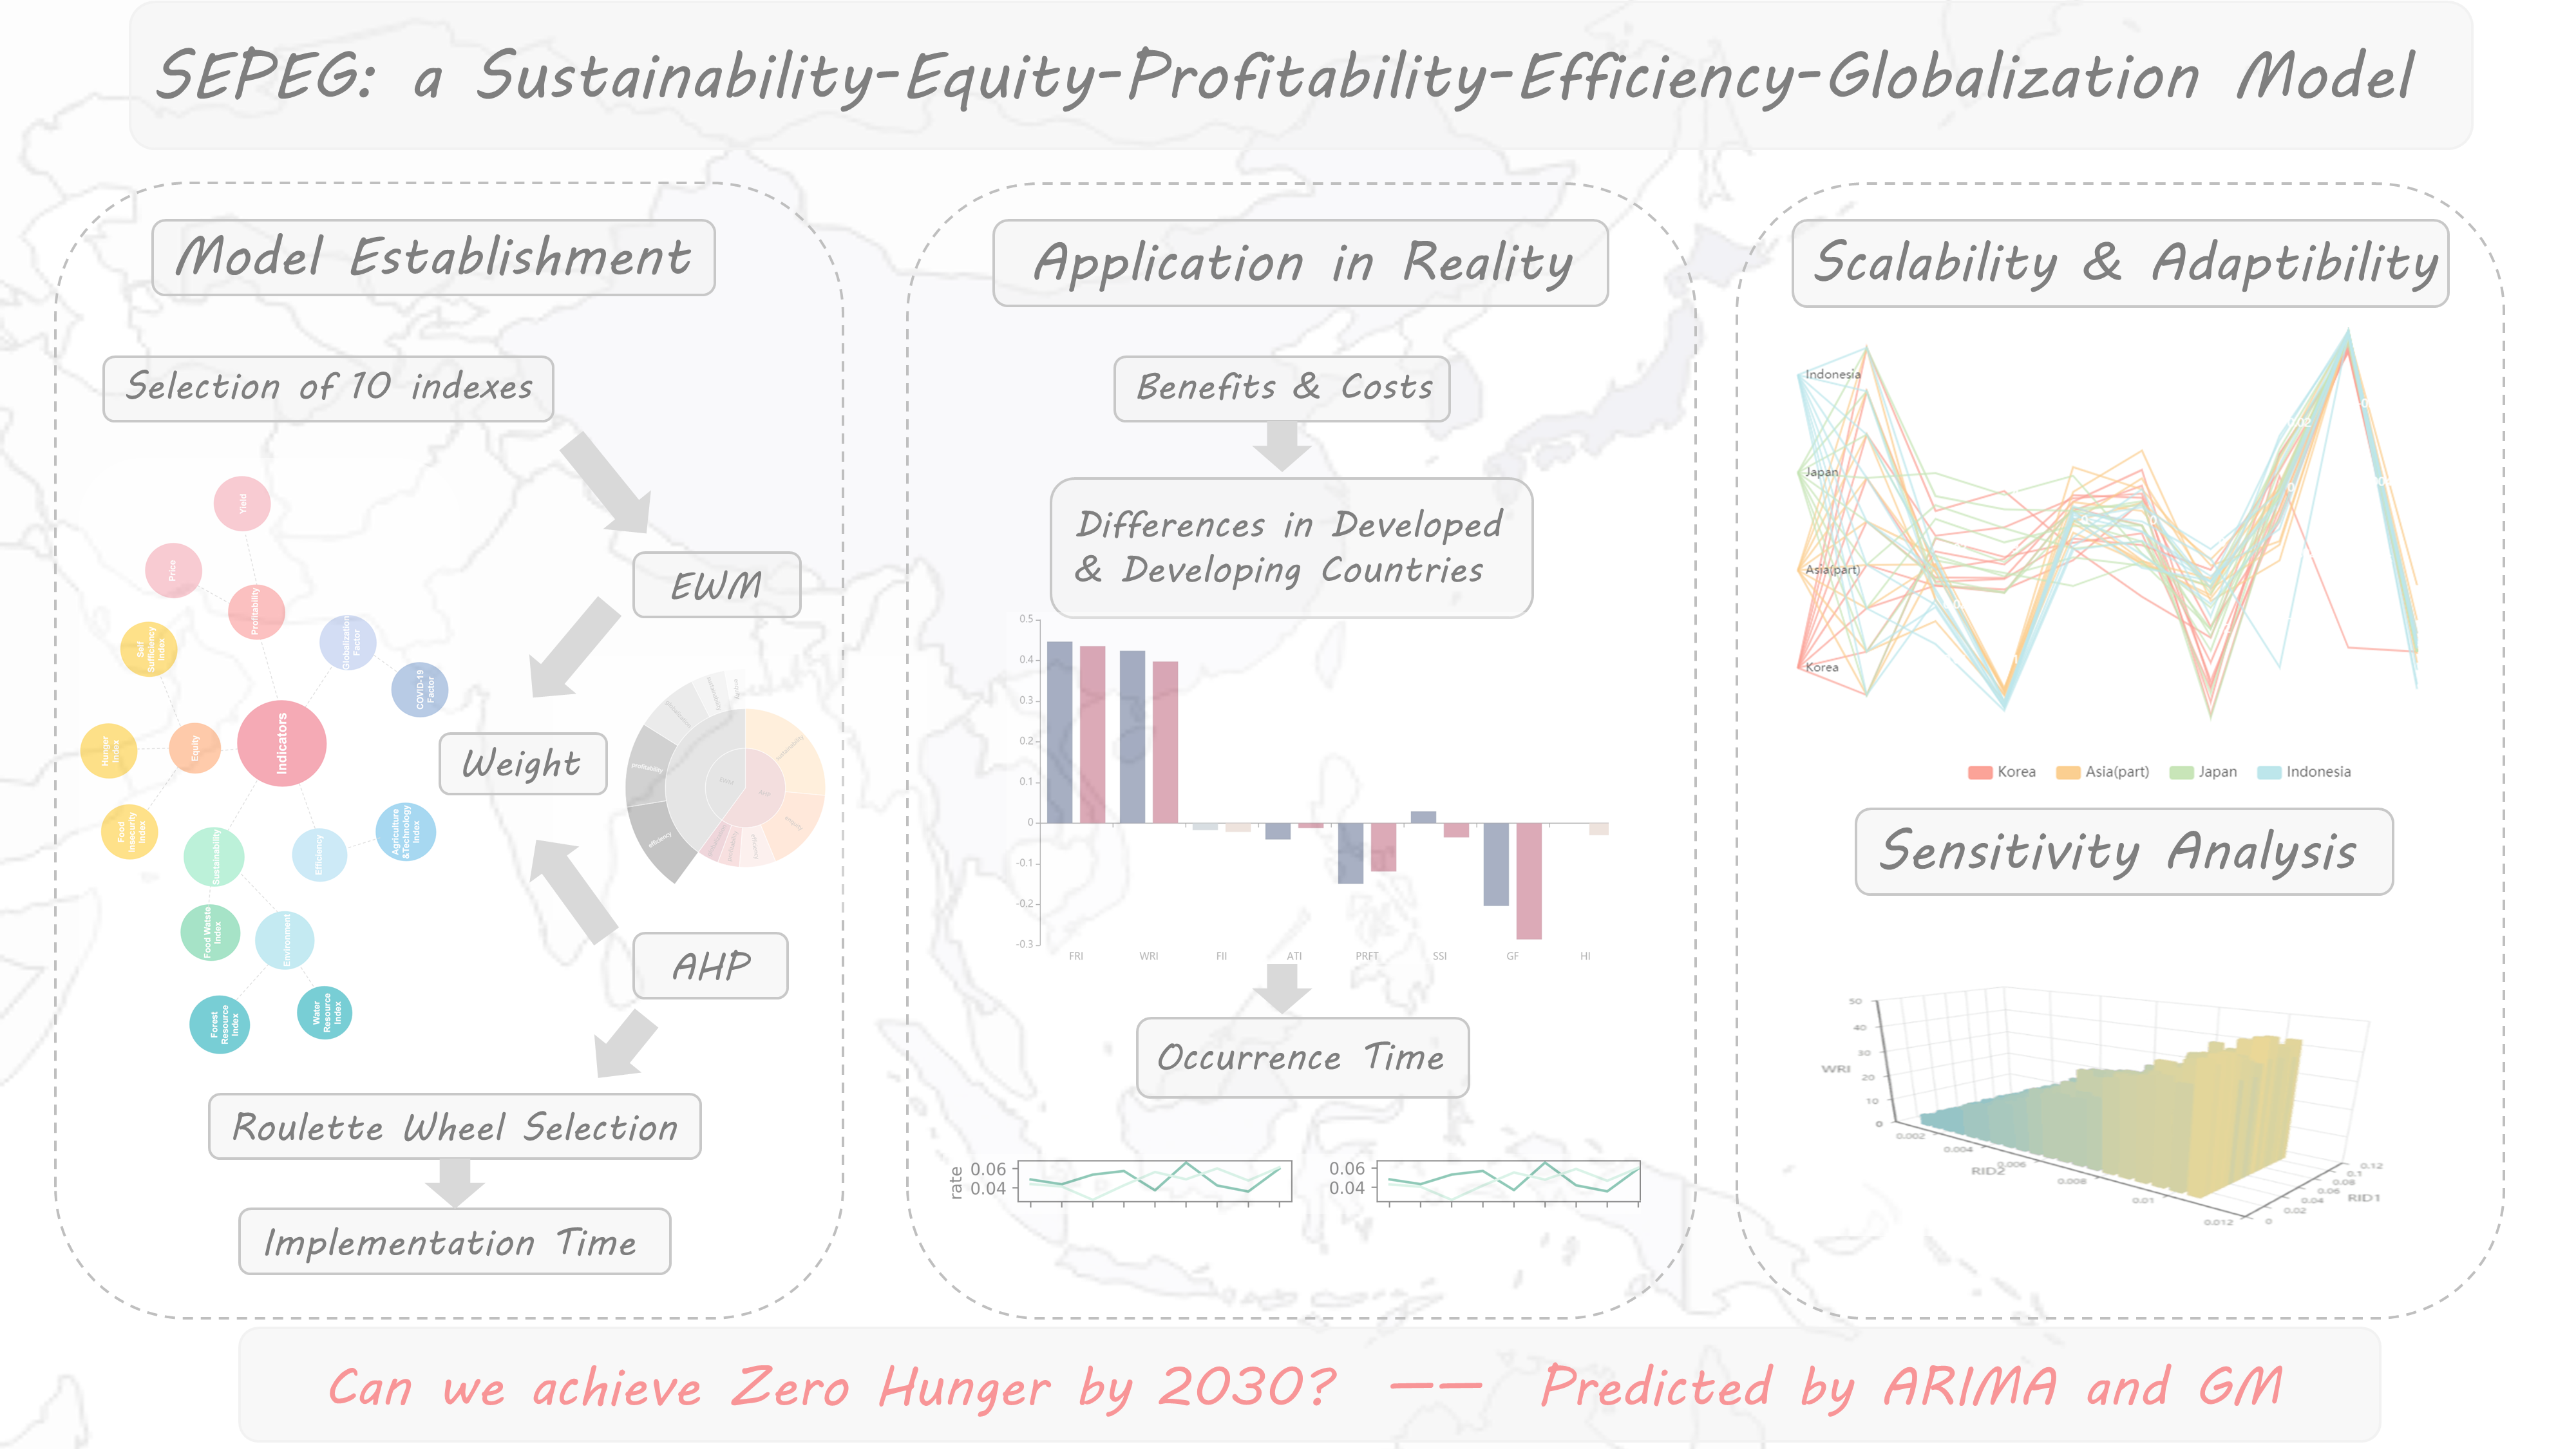
\includegraphics[height=8.34cm]{flowchart.png} 
	\caption{Flow Chart of Our Work}
	\label{fig:eg1}
\end{figure}


 \section{Assumptions And Nomenclature}
 To simplify the model reasonably, we make the following assumptions.
 \begin{itemize}
     \item We assume that the data before 2000 has no impact on today's food systems.
     \item We assume that problems in the food systems of 6 selected Asian countries can be replicated in the world food system.
     \item We assume that the missing parts of the data have no effect on the construction of the model by the process of fitting and random digit.
     \item We assume that the amount of change in five indicators in one day can be added up over the course of a year to indicate changes in priorities for the food system.
     \item We assume that the total amount of regional resources remain constant.
     \item We assume that developed countries have already achieved the goal of Zero Hunger.
     \item We assume that countries with a population of less than 10 million have little impact on the food system of surrounding region where it is located.
 \end{itemize}

 
 \begin{table}[H]
	\centering
	\caption{Notation}
	\begin{tabular}{ c c }
	\toprule
	  Symbol &Definition\\
	\midrule
	$PRFT$ & Profitability (the product of price and yield )\\
	$Loss$ &The decrease of profitability every year \\
	 $HI$ & Hunger Index (the proportion of
the population in hunger) \\	
	 $FII$ & Food Insecurity Index (the proportion of the population hard to access food)\\
	 $SSI$& Self Sufficiency Index (the residual amount of production per resident) \\
	 $FWI$ & Food Waste Index (the proportion of the wasted food)\\
	$FRI$ & Forest Resource Index (a comprehensive measure of forests) \\
	$WRI$ & Water Resource Index (the revenue made by 1 $m^3$ water)\\
	$ATI$ & Agriculture and Technology Index (a comprehensive measure of mechanization) \\
	$GF$ & Globalization Factor\\
	$covid$ & COVID-19 Factor\\
	$Im$ & Imports (the proportion of import trade)\\
	$Ex$ & Exports (the proportion of export trade)\\
	$TU$ & Total Utilization of food\\
	$TS$ & Total Supply of food\\
	$A$ & The judgment matrix in AHP\\
	$a_{ij}$ & The comparative importance in AHP\\
	$P_{ij}$&The proportion of the $i$th element in the $j$th column in EWM\\
	$W_j$ & The weight of the $j$th indicator\\
	$e_j$ & The information entropy in EWM\\
	$g_j$ & The difference coefficient in EWM\\
	$\delta_y$&  The difference between the selected year's index and the next year's\\
	$RID$ & The degree of resource inclination\\
    \bottomrule
	\end{tabular}
	\label{tbl:notation}
\end{table}

 \section{Launch of SEPEG Model}
 \subsection{Selection of Indicators}\label{subsec-indicators}
 The food system is a fairly immense and complex subject that touches every aspect of our daily lives. It includes all processes and infrastructure involved in feeding a population: growing, harvesting, processing, packaging, transporting, marketing, consumption, distribution and disposal of food and food-related items. It also contains the inputs needed and outputs generated at each of these steps, operating within social, political, economic, and environmental contexts\cite{Wiki_foodsystem}. In order to have a deeper understanding of the food systems and obtain a rough outline of our model, several indicators of the food system need to be selected, corresponding to the guiding principle of efficiency, profitability, sustainability, equity and globalization. 
 
 \begin{figure}[H]
	\centering
	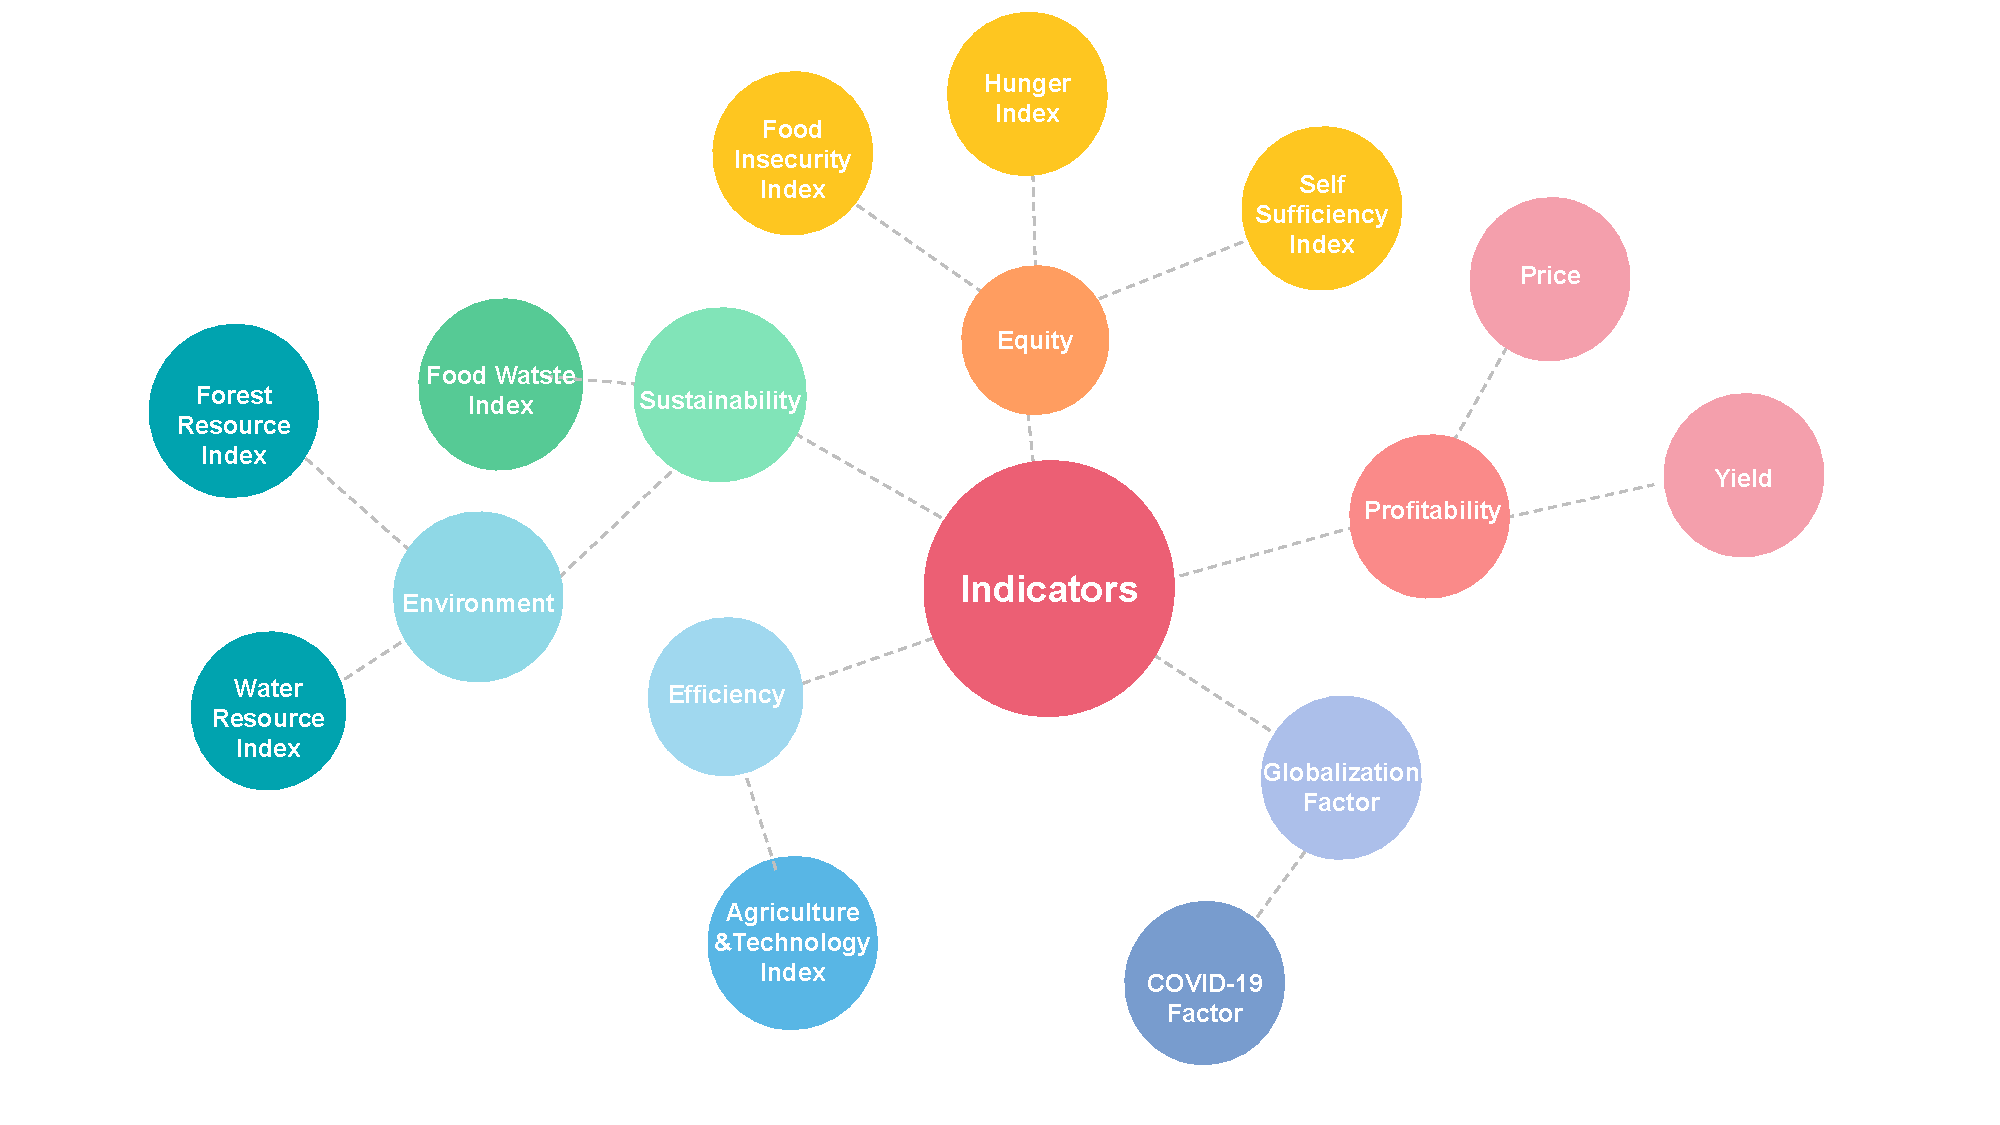
\includegraphics[height=8cm]{Indicators.pdf} 
	\caption{The selection of indicators to evaluate and reprioritize food system.}
	\label{fig:indicators}
\end{figure}
 
 First, the efficiency. It is widely acknowledged that the agricultural mechanization and high technology have greatly boosted the production efficiency of the food system. The \textbf{Agriculture and Technology Index} measures the degree of mechanization and application of advanced technology in different regions, suitable to depict the production efficiency.
 
Second, the profitability. In any case, the maximization of revenue is the eternal pursuit of traders in the food system. We collect the data on agriculture producer \textbf{price} (expressed as US dollars). These are prices received by farmers for primary crops, live animals and livestock primary products as collected at the point of initial sale\cite{price}. Correspondingly, we then need \textbf{yield} (expressed as weight of crops), the full amount of the harvest without the use, to describe the profitability from another angle. 
 
Third, the sustainability. A sustainable food system is one that guarantees food security and nutrition for all without sacrificing the economic and environmental foundations on which future generations depend. This means that it brings broad benefits to society, and that it has a positive or neutral impact on natural resources and the environment. We take two factors in to account, which is food waste and environment. To quantify them, we introduce the\textbf{ Food Waste Index} (expressed as a percentage), the amount of food wasted as a proportion of the total \cite{loss}. To further extend the scale of environmental influences, we sort the \textbf{Forest Resource Index} and the \textbf{Water Resource Index}. The Forest Resource Index is measured through forest area annual net change rate, above-ground biomass stock in forest, proportion of forest area within legally established protected areas, proportion of forest area under a long-term
forest management plan and forest area certified\cite{Forest}. As for the Water Index, we apply the definition of the revenue made by 1 $m^3$ water to describe\cite{water}.

Forth, the equity. Food equity is an expansive concept that all people have the opportunity to grow and to consume sufficient, healthful and affordable foods\cite{food_equity}. Considering that there are still a huge amount of people in the world not disengaging themselves from hunger, we select the \textbf{Hunger Index} as an indicator. It is an estimate of the proportion of the population (expressed as a percentage) whose habitual food consumption is insufficient to provide dietary energy level required to maintain normal activity and a healthy life\cite{hunger_index}. Besides, food security and nutrition are also becoming increasingly serious problems. The \textbf{Food Insecurity Index} provides internationally-comparable estimates of the proportion of the population (expressed as a percentage) facing moderate or severe difficulties in accessing food\cite{insecurity_index}. In order to make the consideration of equity more comprehensive, we further define the \textbf{Self Sufficient Index} by ourselves, which means the residual amount of production per resident after necessary feed use of domestic livestock and food use in one selected country.

Fifth, the globalization factor. In an era of unprecedented globalization, the scope of the food system undoubtedly extents to the entire planet. Considering the fact that it is such a huge system with so many things involved, we bring the \textbf{Globalization Factor} into analysis as Equation \eqref{eq GF}. The ratio of $Im$ to $TS$ shows the proportion of import trade, while the ratio of $Ex$ to $TU$ displays the weight of the export. Since export trade usually can better reflect the country's participation in the global production supply chain than import trade, we give different weights to the two ratios. Thus $k_1$ equals to $0.8$ and $k_2$ is $0.2$. What's more, the black swan event COVID-19 epidemic brings tremendous impacts on global agricultural circulation recently and even for some time in the future, so it is necessary to take the factor $covid$ into consideration \cite{covid}. 

\begin{equation}
\label{eq GF}
GF=\,\, covid \times (k_1\times \frac{Im}{TS}+k_2\times \frac{Ex}{TU}),
\quad \text{where} \quad k_1+k_2=1
\end{equation}

\textbf{Note: All our data and definitions are based on the resources from Food and Agriculture Organization of the United Nations (FAO).}

\subsection{Determination of The Weight}
\label{Sec-weight}
It is sophisticated for us to evaluate the food system appropriately, as there are numerous indexes grouped into five main indicators, which are both objective and subjective. To assess the importance of each indicator as effectively as possible, after data processing, we initially use \textbf{Entropy Weight Method (EWM)} to evaluate the current food system pursuing efficiency and profitability \textbf{objectively} by the given data and then combine \textbf{Analytic Hierarchy Process (AHP)}, a more \textbf{subjective} evaluation method, to further amend the weight of each indicator for the system optimized for sustainability and equity.

\subsubsection{Data Processing}
For future evaluation, we process the data we download from the online database of FAO previously. Considering that Asia is the most populous continent in the world, and includes both developed and developing countries, which can more comprehensively reflect the current situation of the food system, so \textbf{we select countries from Asia as the research object}. According to the data integrity of FAO AMIS system, we further choose 6 Asian countries for study, namely China, Japan, Viet Nam, Thailand, Indonesia and Korea, shown in Figure \ref{fig:world}. (The color depth reflects the per captia GDP.)


 \begin{figure}[H]
	\centering
	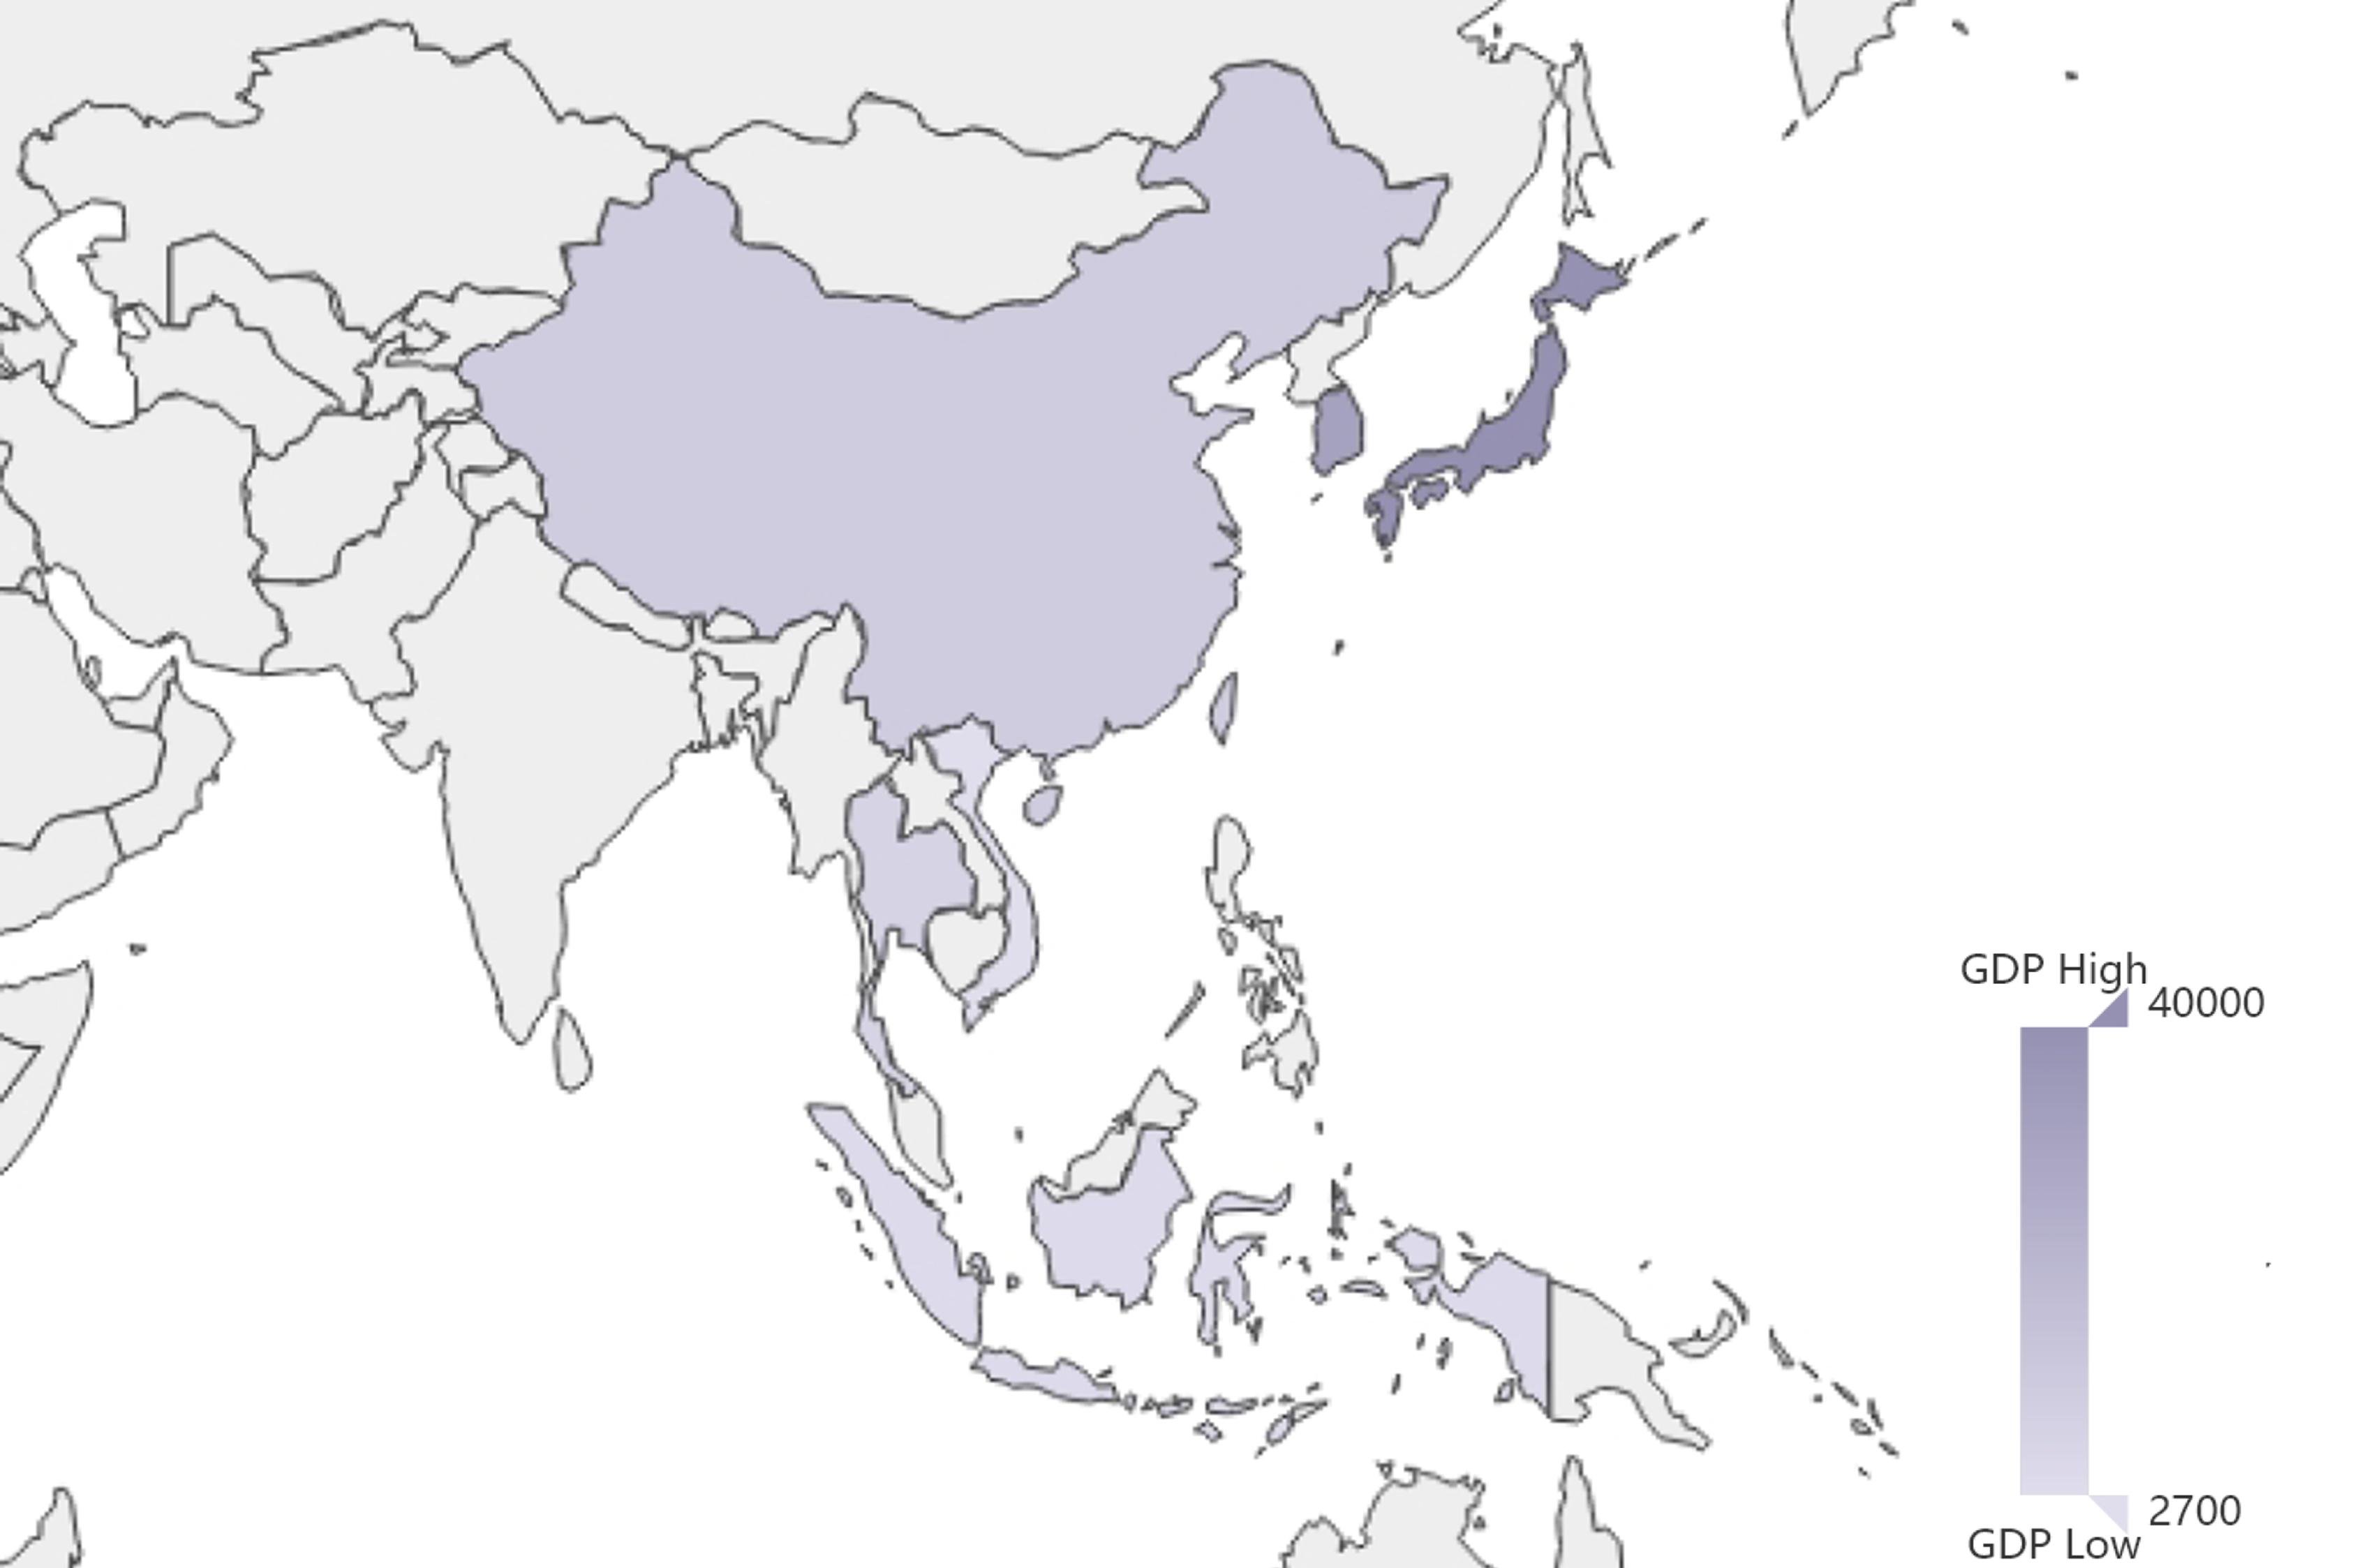
\includegraphics[height=8cm]{Map.png} 
	\caption{The selection of countries.}
	\label{fig:world}
\end{figure}

In Section \ref{subsec-indicators}, there are around nine indexes overall, which means one or more indicators are the combination of different indexes. To simplify the data calculation process, each index of selected indicator are considered equally important to the value of indicator. For example, $WRI$ and $FRI$ play the same role in sustainability. \textbf{Inevitably, some data is found missing in the data set. In this case, we take methods like fitting, random digit and others to fill the blank ones.} For instance, index $HI$ will not be included in the data set when it's value is under $2.5$. So the method of random digit is applied when we are confronted with this situation.

Then, we start to \textbf{normalize the data}. For those indexes who are positively correlated to the final evaluation value, the method of min-max ensure that the data range of the same indes is between $0$ and $1$. While for those who are negatively correlated, they range from $-1$ to $0$ instead, such as $FI$, $FII$ and $FWI$. The process of the data primarily boosts our working efficiency, which greatly alleviates our future work. 

\subsubsection{Objective Evaluation by EWM}
\label{Sec-EMW}
\textbf{Entropy Weight Method} (\textbf{EWM}) is one kind of relatively objective weight-giving method, which can be adopted to verify the weight. The main principle is that the higher the variation degree of indicator, the more useful information reflected, which means the higher this indicator's weight ought to be.

Apparently, $6$ countries and $5$ main indicators are taken into consideration, thus the data has $6$ rows and $5$ variables. Based on the normalized data and Equation \ref{eq EMW1}, we can easily calculate the proportion of the $i$th element in the $j$th column.

\begin{equation}
\label{eq EMW1}
P_{ij}=\frac{x_{ij}}{\sum_1^6{x_{ij}}},
\quad \text{where} \quad j=1,2...,m
\end{equation}

From the definition of information entropy $e_j=-\sum_1^6{P_{ij}}\times \log P_{ij}\div \ln 6$, the difference coefficient of the $j$th variable $g_j=1-e_j$ can be obtained. Thus comes the Equation \ref{Eq EMW2} which measures the weight of the $j$th variable. The weights of five main indicators measured by EWM are shown in Table \ref{tab:weight}.

\begin{equation}
\label{Eq EMW2}
W_j=\frac{g_j}{\sum_1^5{g_j}}
\end{equation}

\subsubsection{Subjective Revision by AHP }
\label{Sec-AHP}
Considering that the final result of EWM  is only based on data, we need to introduce the correction of subjective factors. In this step of sequencing the indicators, we apply \textbf{Analytic Hierarchy Process (AHP)} to judge their importance. The analytic hierarchy process is a structured technique applicable to situations where there is uncertainty and subjective information, allowing experience to be applied in a logical way. This enables us to seriously measure the relative importance between different factors and thus give a standard for ranking 5 major indicators.

According to the reliable literature \cite{AHP} which also use AHP to build a sustainable agriculture, we draw deductive analogy. Resilience of farming systems  is similar to the concept of sustainability, while self-reliance and equity corresponds to the equity. Wise use of resources is regarded as the efficiency of the food system. As for the profitability and the globalization factor, we consider them having the same level of importance. 

To make the hierarchy more authoritative and objective, we refer to the widely adopted data based on some literature \cite{AHPjudge}, where different integers between 1 and 9 represents different comparative importance scale of criteria. 1 is defined as equally important and indicates the importance of both comparative alternatives is equal. 3 is considered as weakly important so experience and judgment weakly tend to prefer one alternative. 5 is strongly important and judgment strongly tend to prefer one alternative. The bigger the value, the more important the factors. Under the actual circumstances of food system, we refer to the data in the literature and carry out the \textbf{judgment matrix}. 

\begin{equation}
\label{matrix:AHP}
A= (a_{ij})=	\left[ \begin{array}{ccccc}
	1 & 2 & 4&5&5 \\
	\frac{1}{2}&1 & 3& 4&4 \\
	\frac{1}{4} & \frac{1}{3} & 1&2&2\\
	\frac{1}{4} & \frac{1}{3} &\frac{1}{2} &1&1\\
	\frac{1}{4} & \frac{1}{3} &\frac{1}{2} &1&1\\
	\end{array} 
	\right ],\quad \text{where}\quad  a_{ij}= \text{comparative importance}
\end{equation}

We then calculate the largest eigenroot and the correspondence eigenvector of the judgment matrix. After normalization, making the sum of each element in the vector equal to 1, we have the weight vector. Each element in the weight vector corresponds to the  AHP weight in Table \ref{tab:weight}. The value is the ranking weight of the relative importance of a factor through AHP method. 

 \begin{table}[h]
 	\centering
 	\caption{The Weight of Indicators}
 	\label{tab:weight}
 	\begin{tabular}{c c c c c c}
 		\hline
 		Variety & Sustainability & Equity & Efficiency&Profitability&Globalization Factor\\
 		\hline
 		EMW Weight &0.1147 &0.0698 & 0.3105&0.2886&0.2165\\
 		AHP Weight & 0.4417 & 0.289 & 0.1229&0.0732&0.0732\\
 		Combined Weight& 0.3109& 0.2013& 0.1979&0.1593&0.1305\\
 		\hline
 	\end{tabular}
 \end{table}

In comparison to the weights gained from the method of EMW, we attach great importance to sustainability and equity superior to other indicators under the guidance of the optimized goal, thus their weights determined by AHP are much higher than others'. Figure \ref{fig:weight1} clearly shows the changes of the five indicators' weights under different methods. The evaluation by EWM is dyed grey to represent objectiveness, while weights calculated by AHP is shown by bright colors.

\begin{figure}[H]
    \centering
    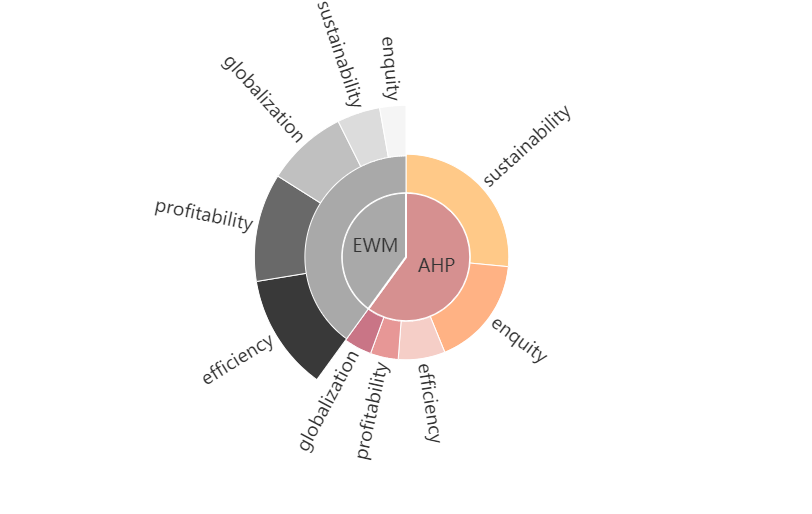
\includegraphics[height=7.5cm]{echarts (11).png}
    \caption{Weights measured separately.}
    \label{fig:weight1}
\end{figure}

Then, in order to obtain one more comprehensive criterion of weight, we integrate both subjective and objective method. As the priorities of the food system are inclined to sustainability and equity, the weights determined by AHP have more reference value. Combined with the value in Section \ref{Sec-EMW} based on the existing data, AHP accounts for $0.6$ while EWM accounts for $0.4$ in the process of determining the mixed weight. Precise value is shown in Table \ref{tab:weight} and visualization is in Figure \ref{fig:weight2} to depict the relationship of the five indicators after modification.

\begin{figure}[H]
    \centering
    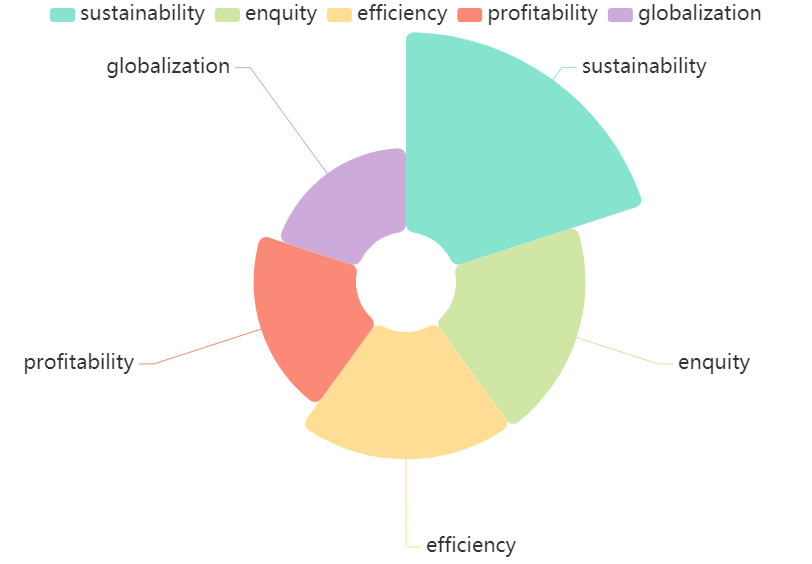
\includegraphics[height=7.cm]{echarts (8).png}
    \caption{Amended weights combining EMW and AHP.}
    \label{fig:weight2}
\end{figure}   

The most outstanding part of our work in this section is the combination of entropy weight method and analytic hierarchy process, so that \textbf{the objective evaluation determined by raw data and subjective revision by human factors are perfectly integrated}. Hence, our final result is both practical and accurate.

\subsection{Further Construction}
\label{Sec-Changes in Optimiaztion}
In Section \ref{Sec-AHP}, we have modified the weights of 5 main indicators of the food system aiming to pursue equity and sustainability. In this part, we mainly focus on the differences triggered by the change of optimization goal, especially the transition of the indexes measuring the five main indicators in one year. With the aid of \textbf{Roulette Wheel Selection} (\textbf{RWS}) and data process, we pave the way for the final establishment of the SEPEG Model.

\subsubsection{Bringing in Roulette Wheel Selection}
\label{Sec-RWS}

\textbf{Roulette Wheel Selection} (\textbf{RWS}) is one classical method based on genetic algorithm, namely proportion selection method, which is broadly adopted to measure the fitness of different individuals. From the perspective of biology, the probability of each individual being selected is related to its fitness to the society, the higher fitness, the bigger chance to be selected. In terms to the food system, we analogy weights of 5 main indicators into the biological individual's fitness, the larger weight signifies the higher probability related work to be carried out. 

In the process of RWS, we define the concept of \textbf{Accumulative Weight ($AW$)} based on the meaning of Distribution Function extracted from the subject \emph{Probability \& Statistics}, which equals to the sum of previous modified indicators' weights. When the normalized random number falls in one interval, we will choose the corresponding indicator and conduct relevant work. Table \ref{tab:RWS Interval} shows the concrete upper and lower bounds of each interval.\textbf{ Considering that our research scale is year and the basic unit is day, so we repeat this process 365 times for every year and 365 values are calculated, that is, each day selects one indicator for further data processing.}

 \begin{table}[h]
 	\centering
 	\caption{Accumulative Weight Interval}
 	\label{tab:RWS Interval}
 	\begin{tabular}{c c c c c c}
 		\hline
 		Variety & Sustainability & Equity & Efficiency&Profitability&Globalization\\
 		\hline
 		$AW$ Interval &(0, 0.31] &(0.31, 0.51] & (0.51, 0.71] & (0.71, 0.87]& (0.87, 1]\\
 		\hline
 	\end{tabular}
 \end{table}

\subsubsection{Operation of Relevant Indicators And Indexes}
After determining the daily indicator in Section \ref{Sec-RWS}, we proceed to explore the changes triggered by this indicator. Before that, we further process the raw data. \textbf{We calculate the difference between the selected year's index ($v$) and the next year's, namely $\delta_y$. The value of the division between difference and the number of days in that year represents Average Daily Change ($\delta_d$).}

In order to describe the influence brought by the selected indicator, we introduce the variable\textbf{ Resource Inclination Degree ($RID$)}. As to the indexes of the selected indicator, their $\delta_d$ will increase due to the resource inclination. The rate of change depends on the value of $RID$. Considering that the data of some indexes are relatively stable and the annual change is not obvious, the revision of $\delta_d$ depends not only on the original $\delta_d$ but also on the index value of the selected year.\textbf{ In this case, $RID1$ is used to measure the factor of the original $\delta_d$ while $RID2$ is for the annual index value.} Besides, on the assumption that the total amount of regional resources remain constant, so the indexes of other indicators will definitely decrease by the same extent. Meanwhile, it is meaningless if the reduction value is below $0$, thus relevant measure is adopted to avoid the emergence of this situation. The Equation \ref{eq RID} shows the detailed calculation rules and measures, and we assign $1\%$ to $RID1$ and $0.1\%$ to $RID2$ according to intuition and experience.

\begin{equation}
\label{eq RID}
\begin{aligned}
    \delta_d&=(1+RID1)\times \delta_d+v\times RID2, \quad \text{for selected indicator}\\
     \delta_d&=\max \left\{ \left( 1-RID1 \right) \times \delta_d\div 4-v\times RID2,\quad0 \right\} , \quad \text{for other 4 indicators}
\end{aligned}
\end{equation}

After having calculated the change of daily indexes, we sum up every day's revised $\delta_d$ of this year. For indicator which contains more than one index, we regard the average $\delta_d$ of the indexes it includes as the measurement of this indicator. The Algorithm \ref{RWS and Further Data Processing} displays the overall process in Section \ref{Sec-Changes in Optimiaztion}. Therefore, we have established a brand-new market system aiming at sustainability and equity, namely \textbf{Sustainability-Equity-Profitability-Efficiency-Globalization Model} (\textbf{SEPEG Model}).


\begin{algorithm}[H]
\label{RWS and Further Data Processing}
	\KwIn{annual forecast data: $D$\ ,\linebreak 
	weight vector:$w=\{w_1,w_2,w_3,w_4,w_5\}$\ ,
\linebreak 
resource inclination degree:$RID_1,RID_2$\ ,\linebreak
maximum forecast days:$maxnum$
	}
	\KwOut{revised annual forecast data:$D_{Revised}$}	
	\BlankLine
	\caption{RWS and Further Data Processing}
	\label{ps}
	obtain each index value of the current year:$v=\{v_1,v_2,v_3,v_4,v_5\}$\;
	obtain the annual change of each index:$\delta_y=\{\delta_{y1},\delta_{y2},\delta_{y3},\delta_{y4},\delta_{y5}\}$ \;
	obtain the daily change of each index:$\delta_d=\{\delta_{d1},\delta_{d2},\delta_{d3},\delta_{d4},\delta_{d5}\}$ \;
	calculate accumulative weight $Q(i)=\sum_{k=1}^{i}w_i$\;
	\For{$count=0$ to $maxnum$}{
		generate a random number $r$ between 0 and $v_5$\;
		\If{$r<Q(1)$}{$priority index=1$\;}
		\Else{$priority index=k$ \ such that $Q(k-1)\textless r \leq Q(k)$\;}
		$\delta_{d\ priorityindex}(count)=\delta_{d\ priorityindex}(count)*(1+RID_1)+v_{priorityindex}*RID_2$\;
		\For{$i=1$ to $5$ and $i\neq priorityindex$}{$\delta_{d\ i}(count)=max\{\delta_{d\ i}(count)*(1-RID_1/4)-v_{i}*RID_2/4,0\}$\;}
	}
	Update $\delta_{d}$ to $D$ to obtain $D_{Revised}$;
\end{algorithm}


\subsection{Implementation Time}
\label{Sec-imp}
When the SEPEG Model is already constructed, it's of vital significance to estimate its implementation time when adopting it in reality. Considering that the biggest change in SEPEG model is the reduction of the profitability's weight, revenue made in the new food system may have a relatively massive drop. \textbf{In view of the resistance of traders and enterprises in the system, the implementation time corresponds to the amount of reduction in revenue.} The less it decreases, the less the resistance and the sooner the new system can be implemented.

\begin{equation}
\label{eq:imp}
    Loss(i)<PRFT(i) \times k, \quad \text{where} \quad i = \text{ordinal number of year}
\end{equation}

Once this inequality condition is satisfied, we assume that the new system can be implemented. $k$ in Equation \eqref{eq:imp} is a constant, depending on the situation in each place. \textbf{The difference between the present point of time and the implementation point of time is defined as the implementation time.} In Section \ref{Sec-when}, we will further discuss the actual situation of the implementation time in selected countries.


\section{Application of SEPEG Model}
\label{sec-App}
With the transfer of the optimization goal, many transformations occur when the SEPEG Model is adopted. After the preliminary determination of EWM and the further revision of AHP, the combined weights of sustainability and equity exceed the other three's weights obviously, which is definitely conductive to indexes related to these two indicators. In this section, we mainly focus on the \textbf{benefits and costs} after we adopt SEPEG Model and reflect on\textbf{ when these visions will take place}.  Meanwhile, it is worth noting that the implementation of the similar policy in different nations may have discrepant effects. So we choose \textbf{Japan and Indonesia} as examples to verify the accuracy of our model and we further give an insight into the comparison \textbf{between developed countries and developing ones} based on the SEPEG Model.

\subsection{Benefits And Costs After Changing Priorities}
\label{Sec-BeneAndCost}
The adjustment of indicator's weight signifies changes in the importance of various indexes. The higher the weight is, the more inclined the resource is to this index, and the system will eventually take on the characteristics of the main indicators \cite{reilly2010managing}. 

As the most important weight, \textbf{sustainability} of the food system definitely grows. Functioning as the basis of human survival and agricultural development, the environment quality will be significantly improved, represented by the Forest Resource Index and Water Resource Index. 

The other relatively significant indicator is \textbf{equity}. There exist obvious distinctions as to the developing situation of every nation, and there also exists a gap between the rich and the poor within the same country. Ensuring the poorest parts of society accessible to necessary food is one vital embodiment of pursuing equity, so our model enhances the equity of food system, and bring benefits to society as more people can enjoy healthy and sufficient food.

\textbf{Profitability} used to be the most important indicator before optimization while it comes to the fourth important in SEPEG Model. As the saying goes, you cannot have your cake and eat it too. On the premise of pursuing environmental and social benefits, the revenue is bound to decrease. As some enterprises' revenue may decline, the vitality of the market will weaken a little bit. This definitely will be the costs the new system has to pay.

The indicator \textbf{Global Factor} measures one nation's participation in the worldwide production trade. Considering the weakened market vitality, the value of the \textbf{Global Factor} may lessen, partly due to the reduction of foreign investment. 

In a nutshell, the SEPEG Model is \textbf{beneficial} to construct a resource-conserving and environmentally-friendly society and reduce the food insecurity. However, the \textbf{cost} of our system lays in that the income of some enterprises may decrease and have a negative impact on worldwide trade. In Section \ref{Sec-Char}, we will apply our model in two countries and obtain the data, therefore we can evaluate benefits and costs combined with the real situation. 



 \subsection{Characteristics in Developed Countries And Developing Countries}
 \label{Sec-Char}

In Section \ref{Sec-BeneAndCost}, we obtain a general outline of the benefits and costs brought by the change of priorities. In this section, considering that different regions have different levels of development, the scope of our discussion are divided into 2 parts, the developed and developing countries. We select two Asian countries, Japan and Indonesia to apply our model. After obtaining the data of corresponding indicators, we will analyze the characteristics and summarize the \textbf{commonalities and differences} according to their conditions.

When applying our model, we choose 8 indexes for analysis, namely $FRI$ for the Forest Index, $WRI$ for the Water Resource Index, $FII$ for the Food Insecurity Index, $ATI$ for the Agriculture and Technology Index, $PRFT$ for profitability, $SSI$ for the Self Sufficiency Index, $GF$ for the Globalization Factor, $HI$ for the Hunger Index. Considering there is a serious lack of data for the Food Waste Index, so we dismiss its function. Besides, $PRFT$ is expressed as the product of price and yield. After processing data from Japan and Indonesia, we use SEPEG model to obtain the value of various indexes in 2030. Then we compare these data with prediction of raw data in 2030 through time series analysis and normalize the change of their value, shown in Figure \ref{fig:DC} \textbf{(Note: This Figure shows the growth rate rather than the original level. Dark pillars represent positively related indexes, while light pillars represent negatively related indexes)
}
\begin{figure}[H] 
	\centering
	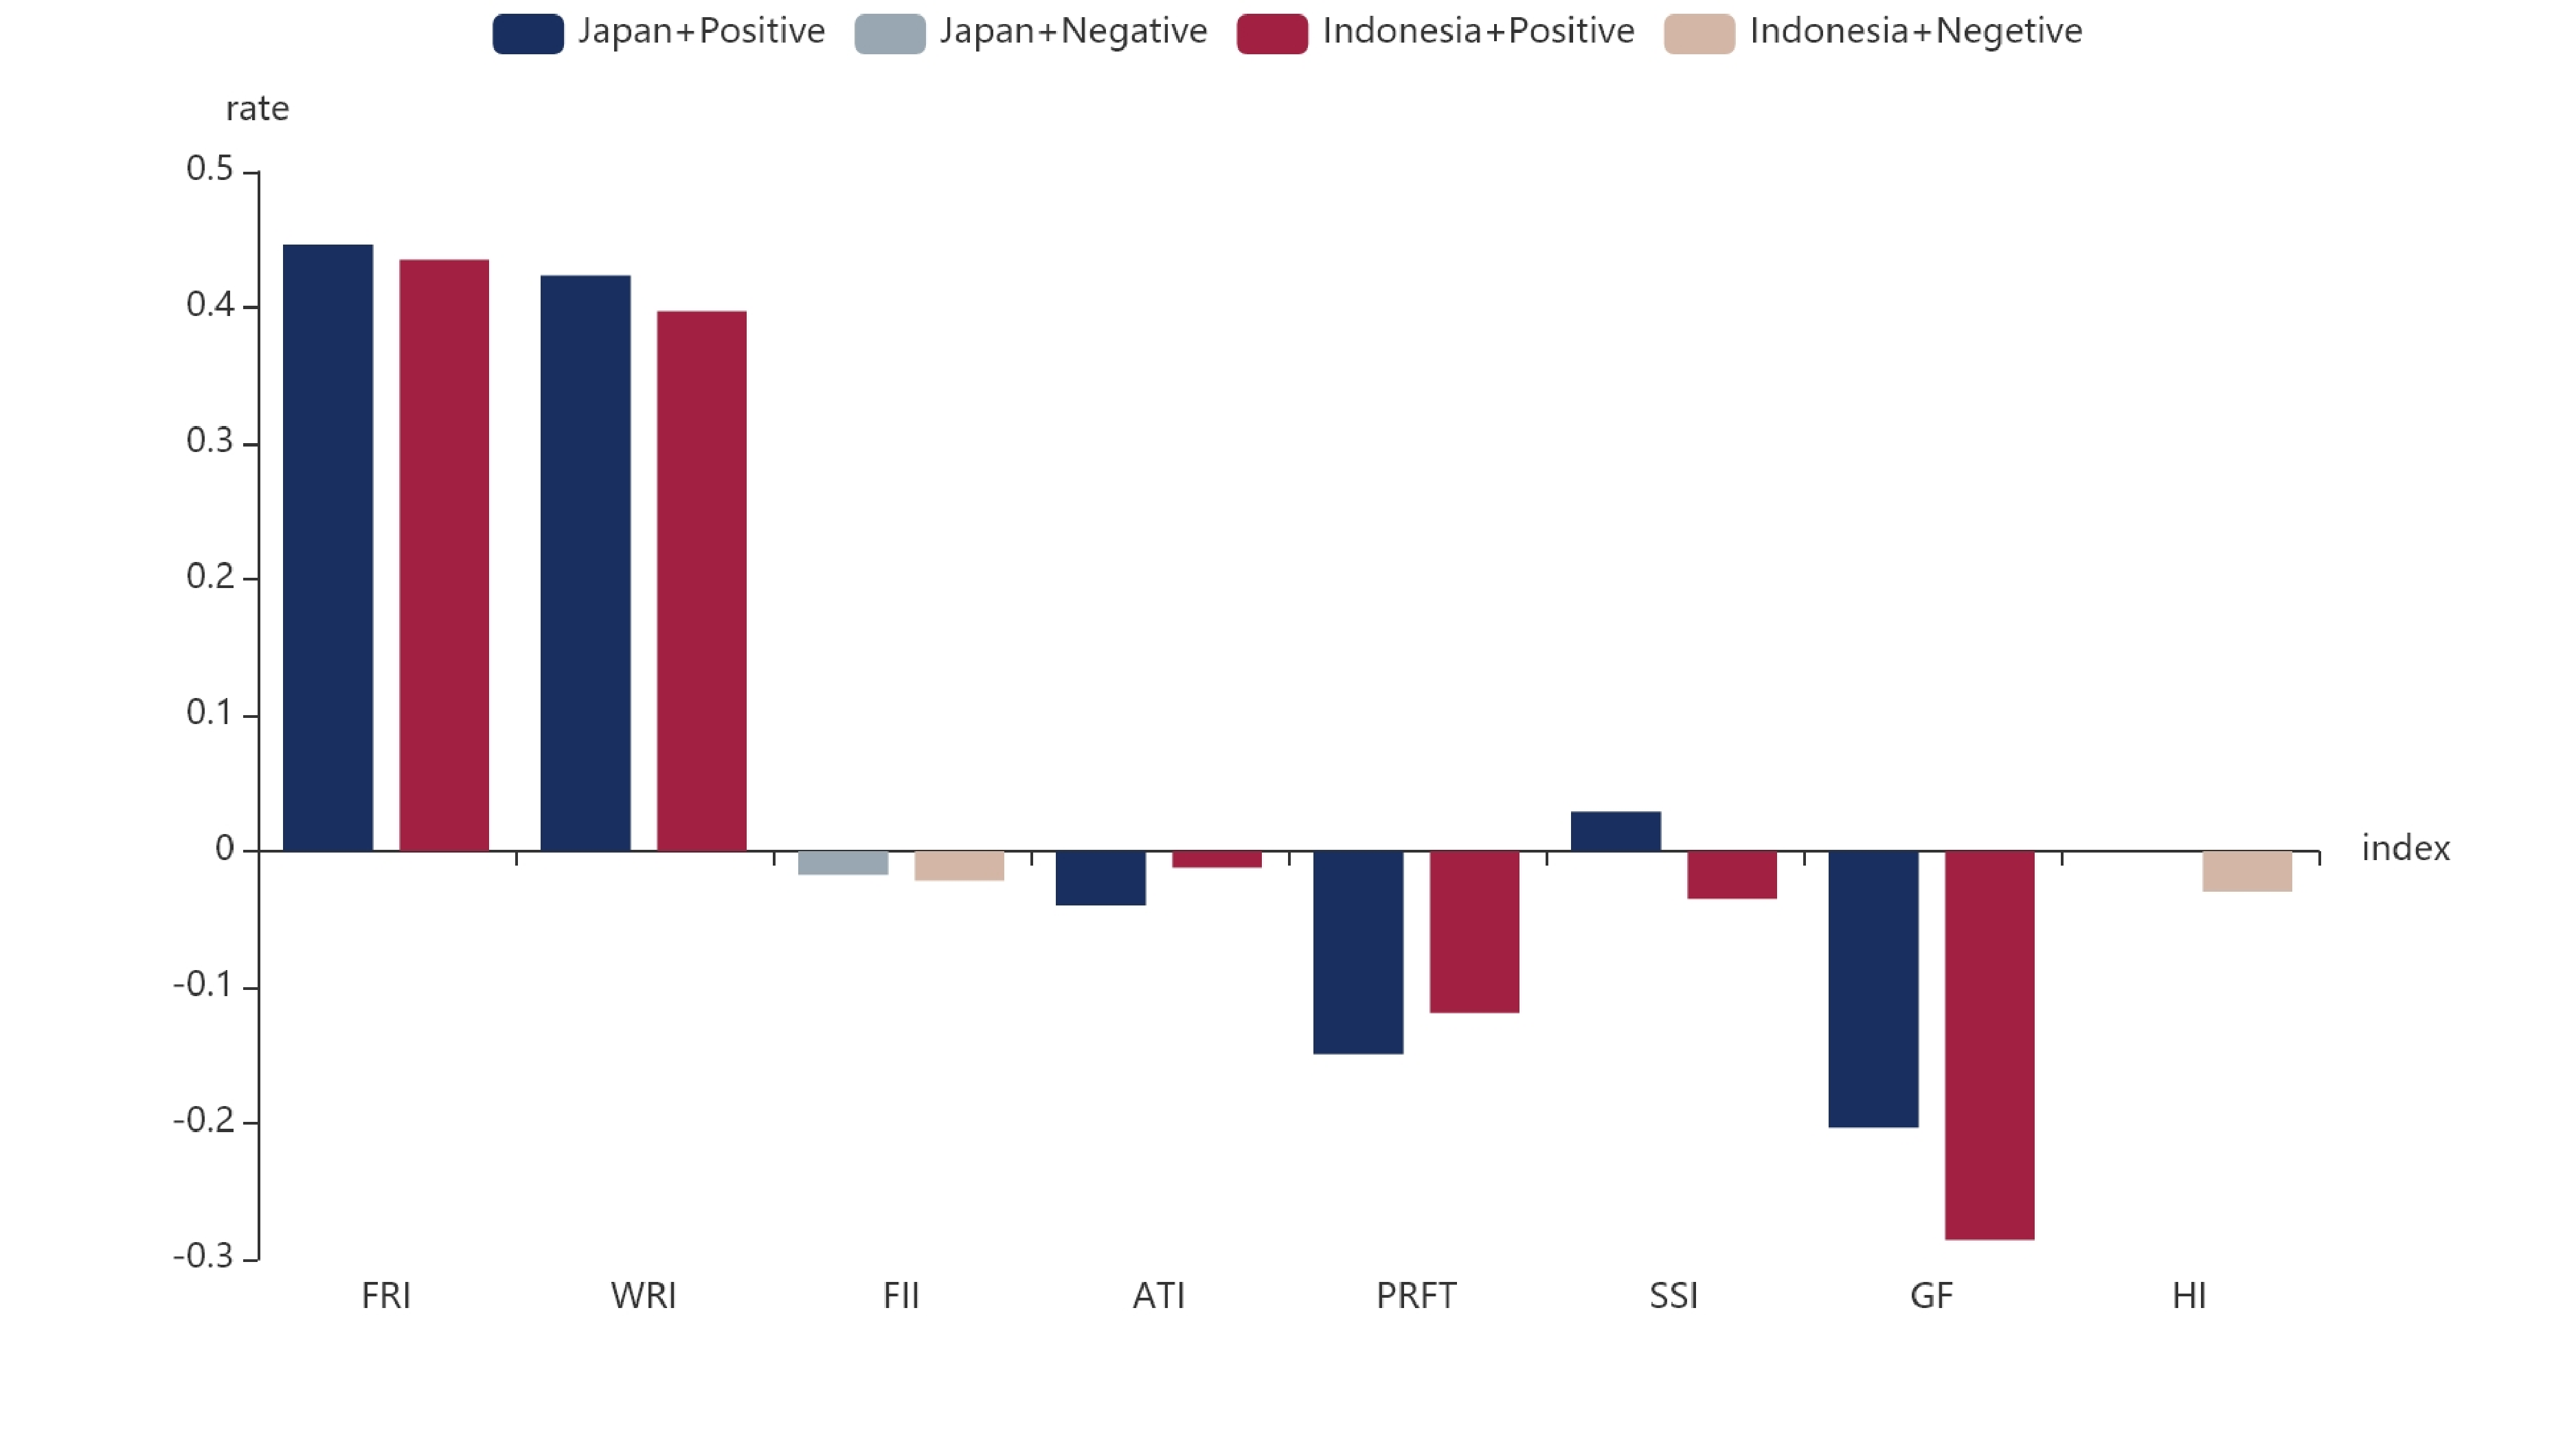
\includegraphics[height=8.5cm]{bar.pdf} 
	\caption{Changing rate of indexes in two countries after normalization in SEPEG model.}
	\label{fig:DC}
\end{figure}

From Figure \ref{fig:DC}, we can generally summarize the following \textbf{similarities} in both countries.

Because of our model's emphasis on sustainability, apparently, the index $FRI$ and $WRI$ in both countries have a huge growth rate, thus boosting to build a \textbf{resource-conserving and environmentally-friendly society.} This is definitely beneficial for the future development of the food system as our environment is improved.

The level of $HI$ and $FII$ decrease, which signifies \textbf{the robustness of the country's food system and the capability to cater to citizens' growing material demands.} Meanwhile, the degree of food self sufficiency remain stable, indicating that the SEPEG system is helpful to solve the problem of food equity in both countries. 
 
The Agriculture and Technology Index has a extremely small reduction, while the overall efficiency maintain stability. In general, \textbf{the degree of technology and agricultural mechanization is stable} the food system function in a relatively efficient way.
 
However, the costs is apparent as well. The profitability decline greatly, at the expense of the interests of some enterprises. \textbf{The vitality of the market may be weakened and foreign investment decreased. }The globalization factor also has a huge rate of reduction. \textbf{It can be understood as the COVID-19 spreads around the world, trade between different countries is obstructed \cite{covid-19}. }
 
 Next, we will focus on the \textbf{differences} between the developed countries and developing countries. 4 indexes show the difference, while other 4 indexes are generally similar. 
 
 Compared with developed country Japan, the increasing range of two sustainability indexes $FRI$ and $WRI$ in developing country Indonesia is not that great. \textbf{This is because that the developed countries themselves attach great importance to the environment, while  developing countries focused on development relatively more as their environmental vegetation is better.} For the Water Resource Index $WRI$, developed countries also show its advance, since their water can create more revenue due to advanced technology.
 
As for the Hunger Index, it only declines in developing countries. Considering that developing countries can still reduce hunger, the range of reduction is generally satisfying. The hunger index in developed countries is already below 2.5, so in Figure \ref{fig:DC} the $HI$ of Japan is 0. From the point of view of hunger, \textbf{SEPEG model displays its superiority in improving the food equity.}

For the costs, the profitability $PRFT$ of both countries reduce greatly, while developed countries decline more and developing countries decline gently.\textbf{ This indicates that our SEPEG model protects the economic interests of developing countries when they are not prosperous enough.}

Other 4 indexes, namely $FII$, $ATI$, $SSI$ and $GF$, are generally similar in two countries, which shows the stability and reliability of our SEPEG model from other aspects.
 
 
\subsection{When Would They Occur?}
\label{Sec-when}

After the evaluation of benefits and costs, it's natural to query when would they occur? Firstly, according to the definition of implementation time in Section \ref{Sec-imp}, we should work out the general time of our SEPEG model to be implemented. In order to adapt to the real situation in Japan and Indonesia, we set the value of $k$ equal to $0.1$ in Equation \eqref{eq:imp}.

 \begin{table}[h]
 	\centering
 	\caption{The Profit And Loss Predicted by SEPEG Model}
 	\label{tab:imp}
 	\begin{tabular}{c c c c c}
 		\hline
 	Country	&1$st$ Year Profit &  1$st$ Year Loss &2$nd$ Year Profit &2$nd$ Year Loss\\
 		\hline
 		Japan &16739.98 &511.33 & 16804.65&125.56\\
 		Indonesia& 14359.84& 278.19&14823.06&35.93\\
 		\hline
 	\end{tabular}
 \end{table}

From Table \ref{tab:imp}, we find out that 1$st$ year loss of both countries is less than 0.1 times profit, which means that the 1$st$ loss is beyond the scope that traders and enterprises in the food system can bear. However, in the 2$nd$ year, the loss satisfies the demand. \textbf{Therefore we obtain the implementation time which is 1 year.}

Then, in order to refine the timing of benefits and costs corresponding to different indexes, we carry out Figure \ref{fig:line} to depict the changing rate of indexes in different years. \textbf{Based on the analysis of the variation in 8 indexes, we generally classify them into 4 types, for different types of indexes has different features while changing in the course of 9 years.}

\begin{figure}[H]
	\centering
	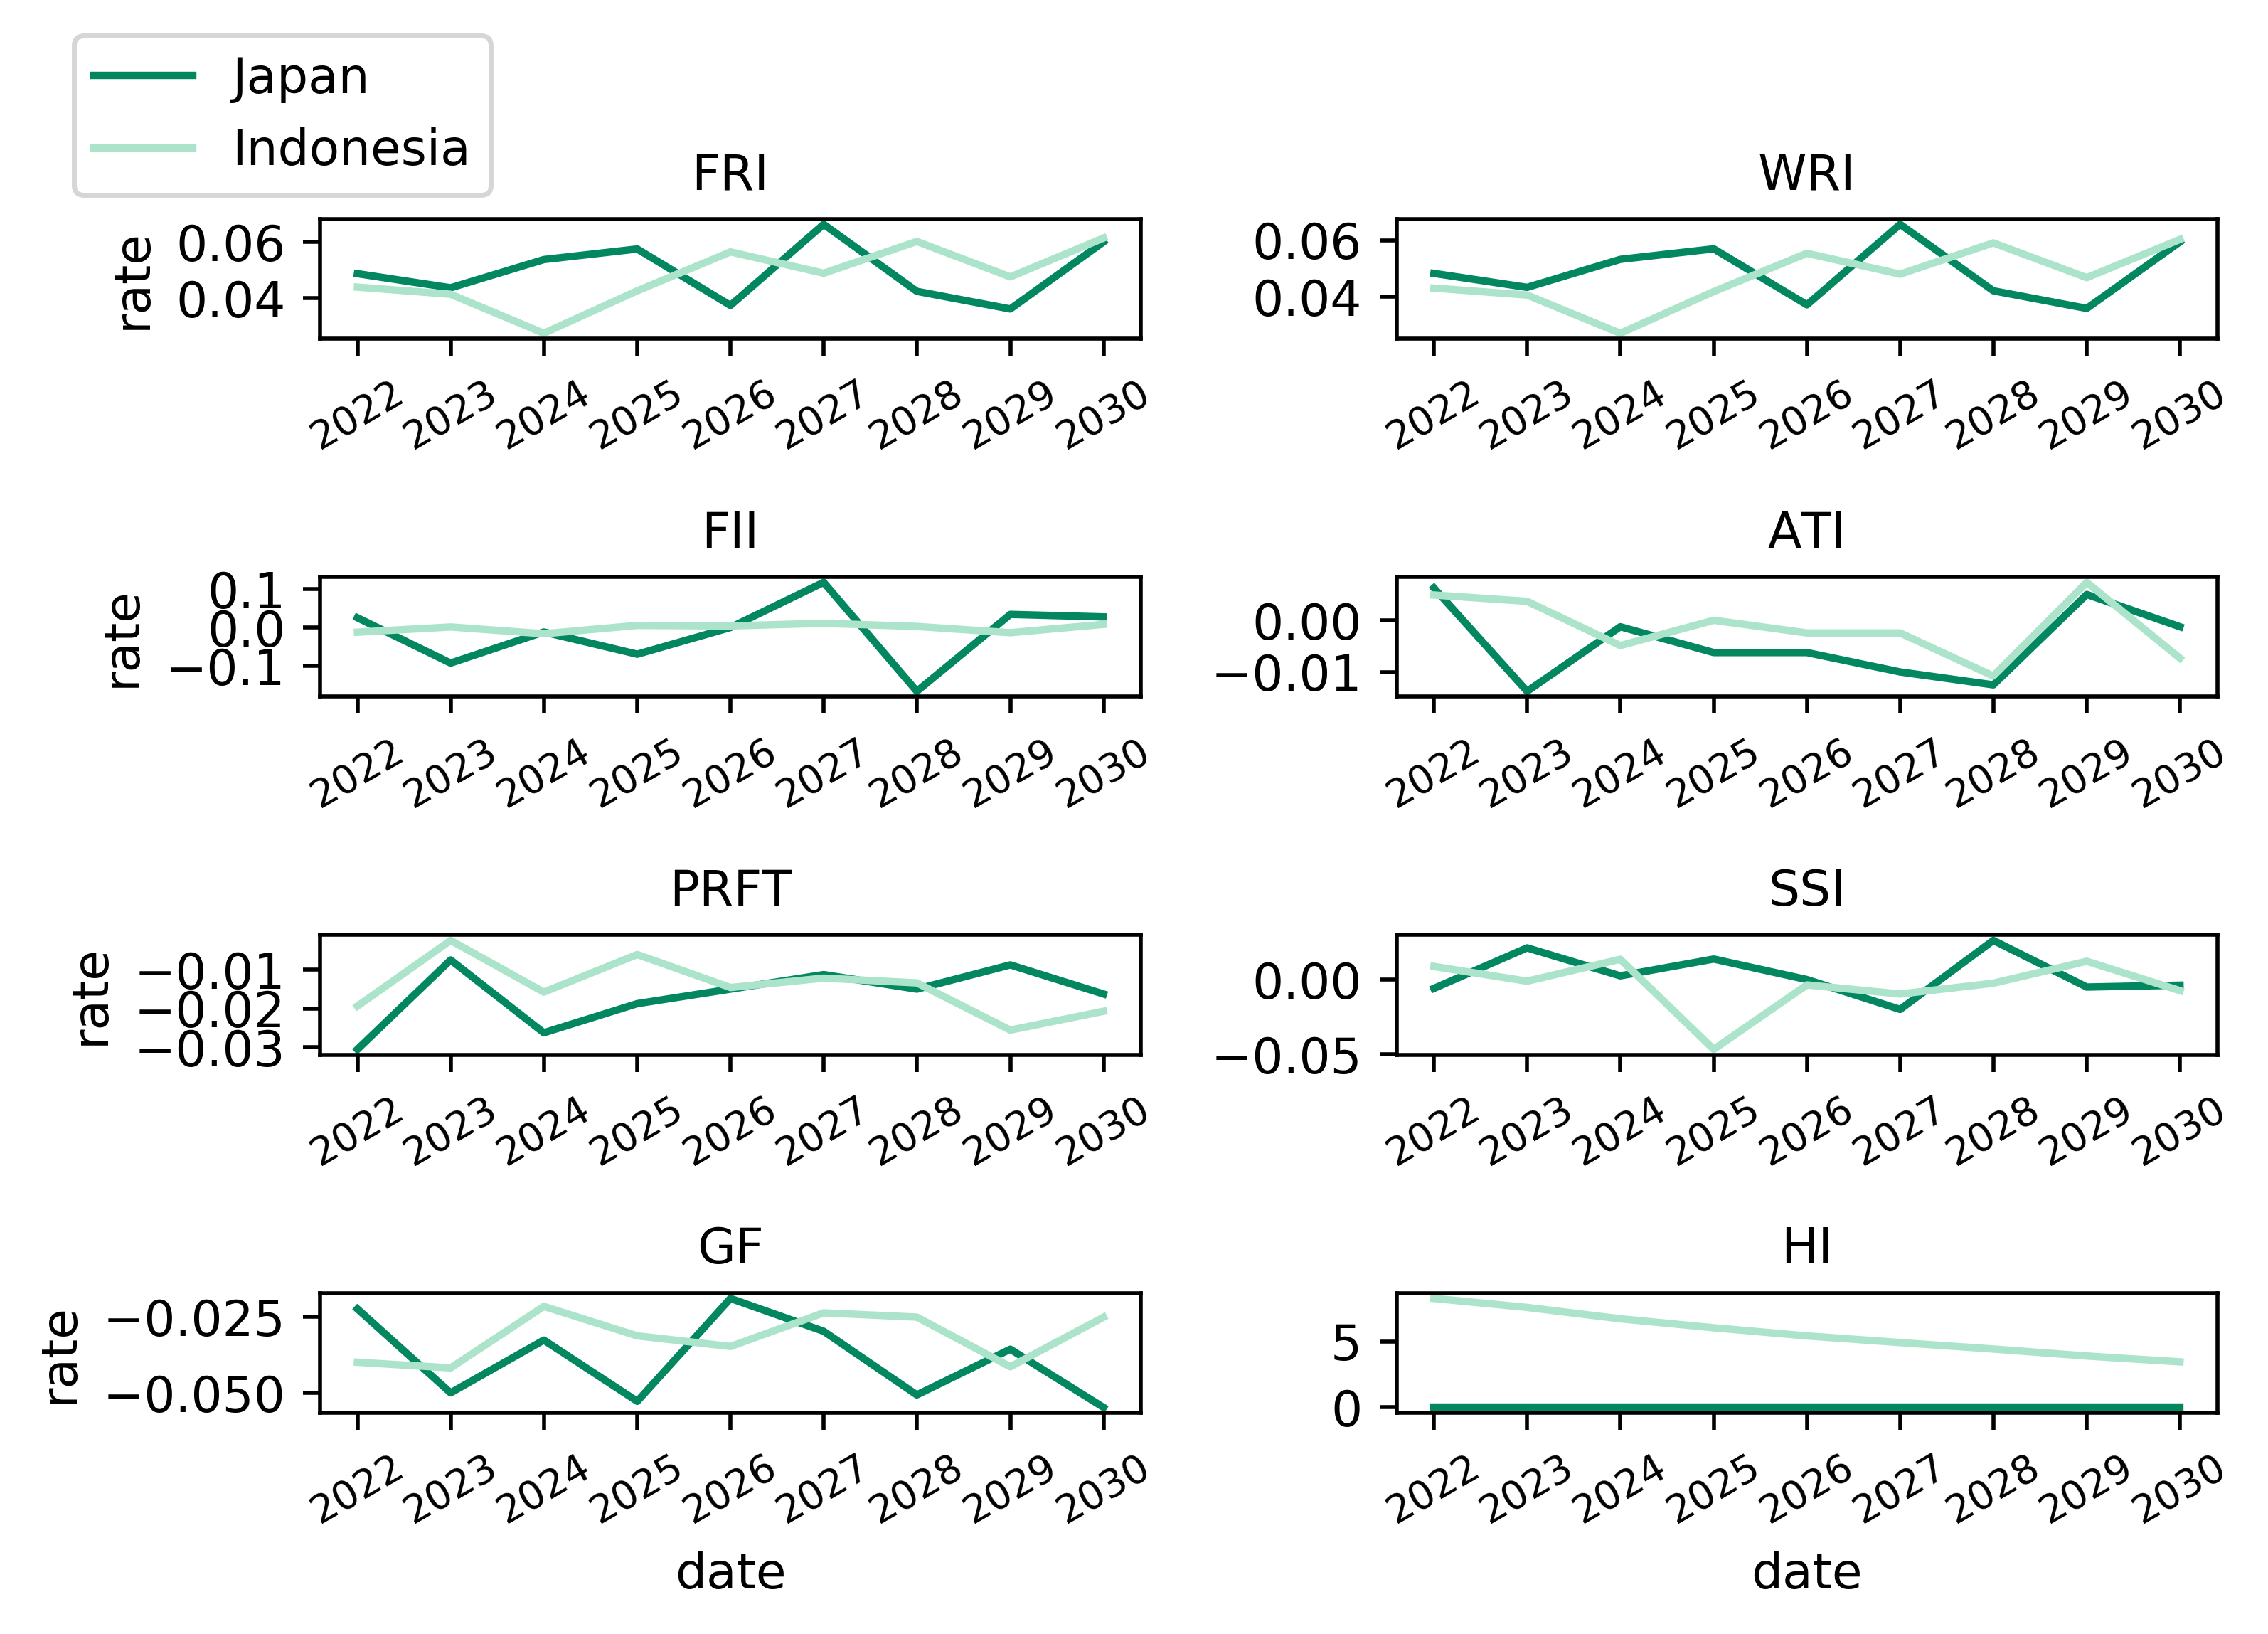
\includegraphics[height=9cm]{line.png} 
	\caption{Changing rate of indexes in different years.}
	\label{fig:line}
\end{figure}

\textbf{Firstly, the indexes whose variation trend is upward steadily will lead to prompt benefits as soon as the optimized system is implemented. }In Figure \ref{fig:line}, it's clear that the Forest Resource Index $FRI$ and the Water Resource Index $WRI$ are continuously rising. Obviously, when the weight of the sustainability is enhanced in Section \ref{Sec-weight}, two indexes subordinate to it correspond with its momentum of rise. In other words, the results of environmental improvement and sustainable development can be seen year by year.

\textbf{Secondly, the indexes which drop apparently will also bring about costs immediately.} For example, the profitability $PRFT$ have a significant reduction compared with other indexes in our SEPEG model. This indicates that the impact of lessening the pursuit of profits can happen in a very short time, even less than a year.

\textbf{Thirdly, the fluctuating indexes which have a general upward trend can bring both benefits and costs depending on the year we select. }Take the Self Sufficiency Index $SSI$ as an example, it varies in uncertain terms, sometimes increasing and sometimes decreasing. Therefore, the benefits and costs can occur at any time, but the benefits are more likely to occur.

\textbf{Fourthly, the results of undulating indexes which have a general downward trend are also uncertain, depending on the given circumstance. }However, the possibility of costs is greater. The Globalization Factor $GF$ can serve as an example, it is undulating but more likely to drop. This indicates that globalized trade is basically stable, but there may be a small decline at an uncertain time.

In conclusion, after working out the implementation time of SEPEG model, we obtain the cardinal number of time. Then, the time that benefits and costs occur corresponds to the feature of the index, that we need to analyze the specific situation.

\section{Can We Achieve Zero Hunger by 2030?}
When the little boy in Africa flashes his big, clear eyes on his thin cheeks, we know that Zero Hunger is a common goal for all human beings in the world. Five years ago, the world pledged to end hunger in all its forms. Now, five years later, do we have a good momentum to complete the mission or are we still lagging behind in achieving our goals?  

In the following section, we will analyze the problem using the time series model from the perspective of two indexes, namely \textbf{the Hunger Index} and \textbf{the Food Insecurity Index}. Considering that the range of data is too large, we select the developing country Indonesia for deeper research according to the data from 2001 to 2018. As Indonesia is a relatively underdeveloped country and the average life quality of people there is poor, it can be regarded as the microcosm of countries fighting against hunger and poverty. Take it as an example,  we can measure progress towards Zero Hunger in those backward countries, which is the most important part of achieving Zero Hunger.

In order to characterize the trend of time series and accommodate the fluctuations more comprehensively, we decide to use \textbf{Autoregressive Integrated Moving Average (ARIMA)} and \textbf{Grey Forecast Model (GM)} together to make predictions.


\subsection{Prediction of Hunger Index by ARIMA}

In Section \ref{subsec-indicators}, we define the \textbf{Hunger Index} as the the proportion of the population whose habitual food consumption is insufficient to provide dietary energy level required to maintain normal activity and a healthy life. Obviously, it's an intuitive indicator of hunger. \textbf{According to the standard of FAO, when $HI$ decreases to 2.5, we deem that this country achieves the goal of Zero Hunger.}

In consideration of the circumstance, we probe into a generative model Autoregressive Integrated Moving Average (ARIMA) to characterize the historical evolution and make predictions in time series. ARIMA is a generalization of AR(autoregressive model), MA(moving average model) and difference method. This technique is theoretically and statistically sound in its foundation, only needing to make very few assumptions. In addition, the model is simple and requires only endogenous variables without the help of other exogenous variables. Equation \eqref{Eq:ARIMA} shows the  mathematical formula.
\begin{equation}
\label{Eq:ARIMA}
y_{t}=C+\sum_{i=1}^{p} \gamma_{i} y_{t-i}+\epsilon_{t}\left(1-\sum_{i=1}^{p} \varphi_{i} L^{i}\right)(1-L)^{d} X_{t}=\delta+\left(1+\sum_{i=1}^{q} \theta_{i} L^{i}\right) \varepsilon_{t}
\end{equation} 

where
\begin{itemize}
\item $C$ is the constant term.
\item $\epsilon_{t}$ is the random error of and its average is assumed to  equal 0.
\item $\gamma_{i}$ is the auto-correlation coefficient. 
\item $L^i$ is the lag operator.
\item $p$ is the order (number of time lags) of the autoregressive model.
\item $q$ is the order of the moving-average model.
\item $d$ is the degree of differencing (the number of times the data have had past values subtracted).
\end{itemize}

With the help of SPSS, a powerful statistical analysis software, we obtain the value of parameters, $p=2$, $q=0$, $d=1$. The final result of ARIMA(2,1,0) is shown in Figure \ref{fig:arima}, where we can see that the fitting is extraordinary, that the raw data and the forecast are almost completely consistent. \textbf{However, according to the Hunger Index in the current food system, $HI$ obviously can't reach 2.5 in the year of 2030, which indicates that the grand goal of UN can't be achieved before the deadline.
}
\begin{figure}[H]
    \begin{minipage}[c]{0.5\textwidth}
       \centering
       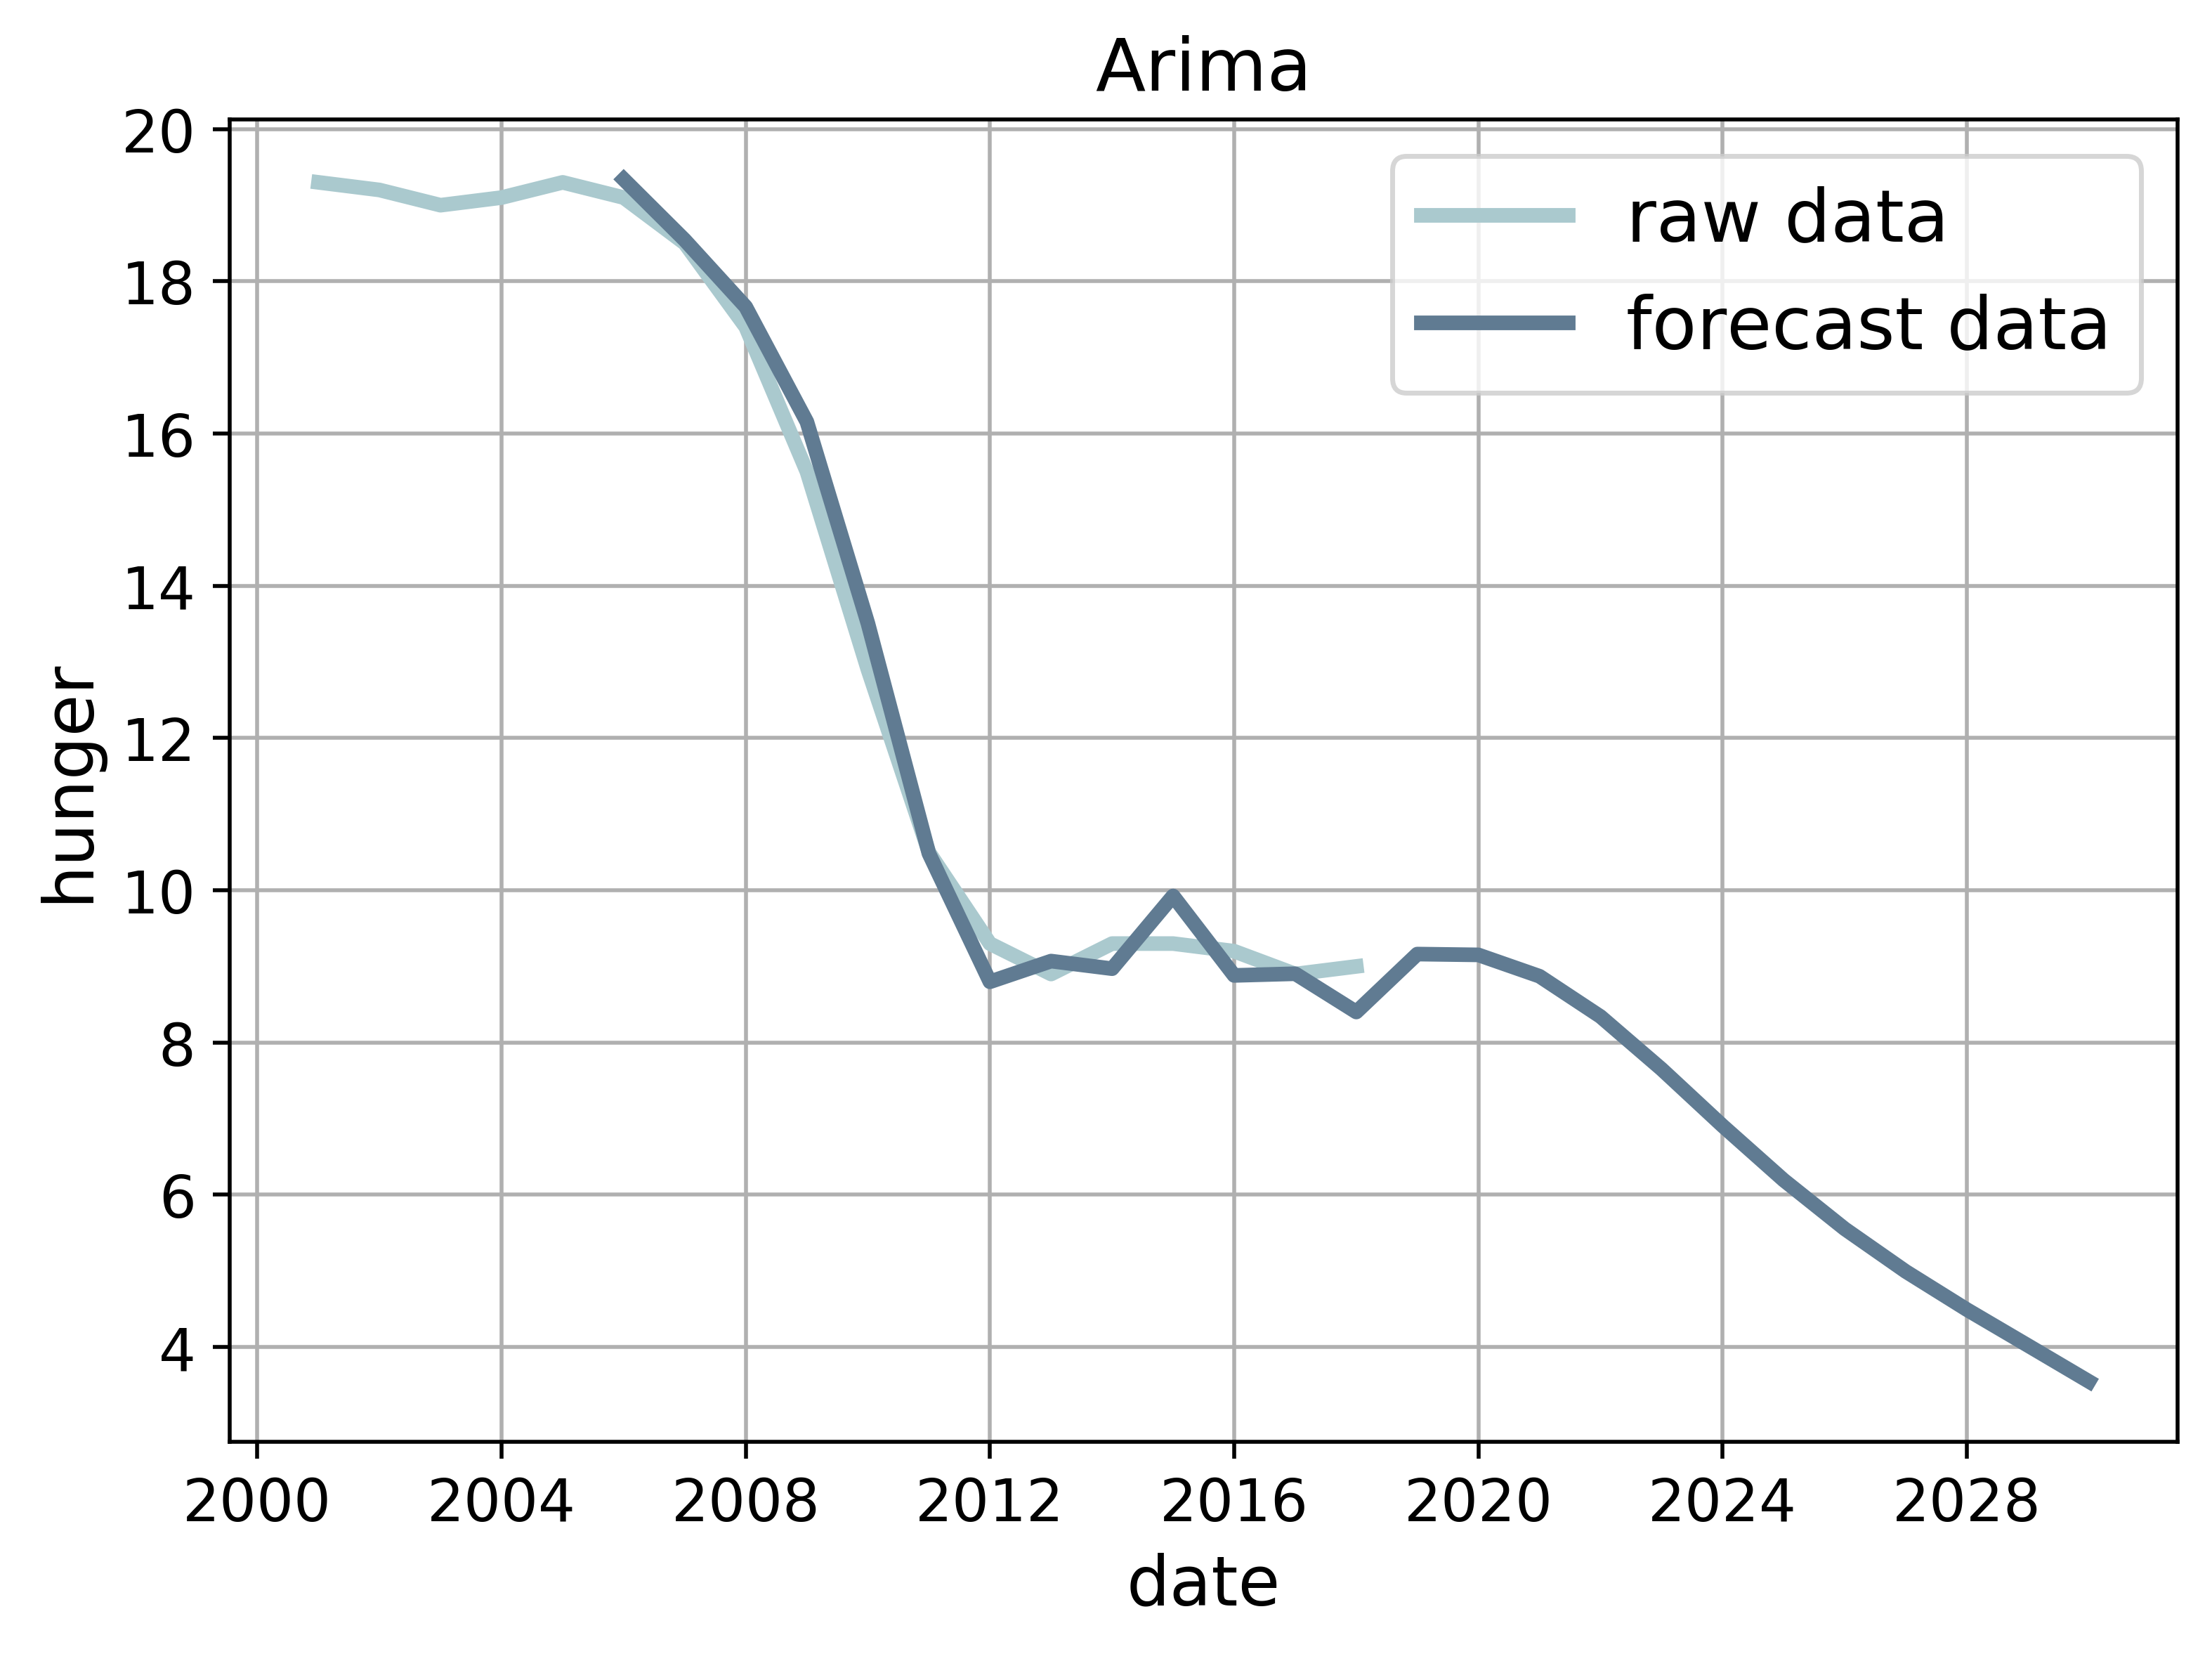
\includegraphics[height=6cm]{arima.png}
       \caption{Prediction of $HI$ by ARIMA.}
       \label{fig:arima}
       \end{minipage}
    \begin{minipage}[c]{0.5\textwidth}
       \centering
       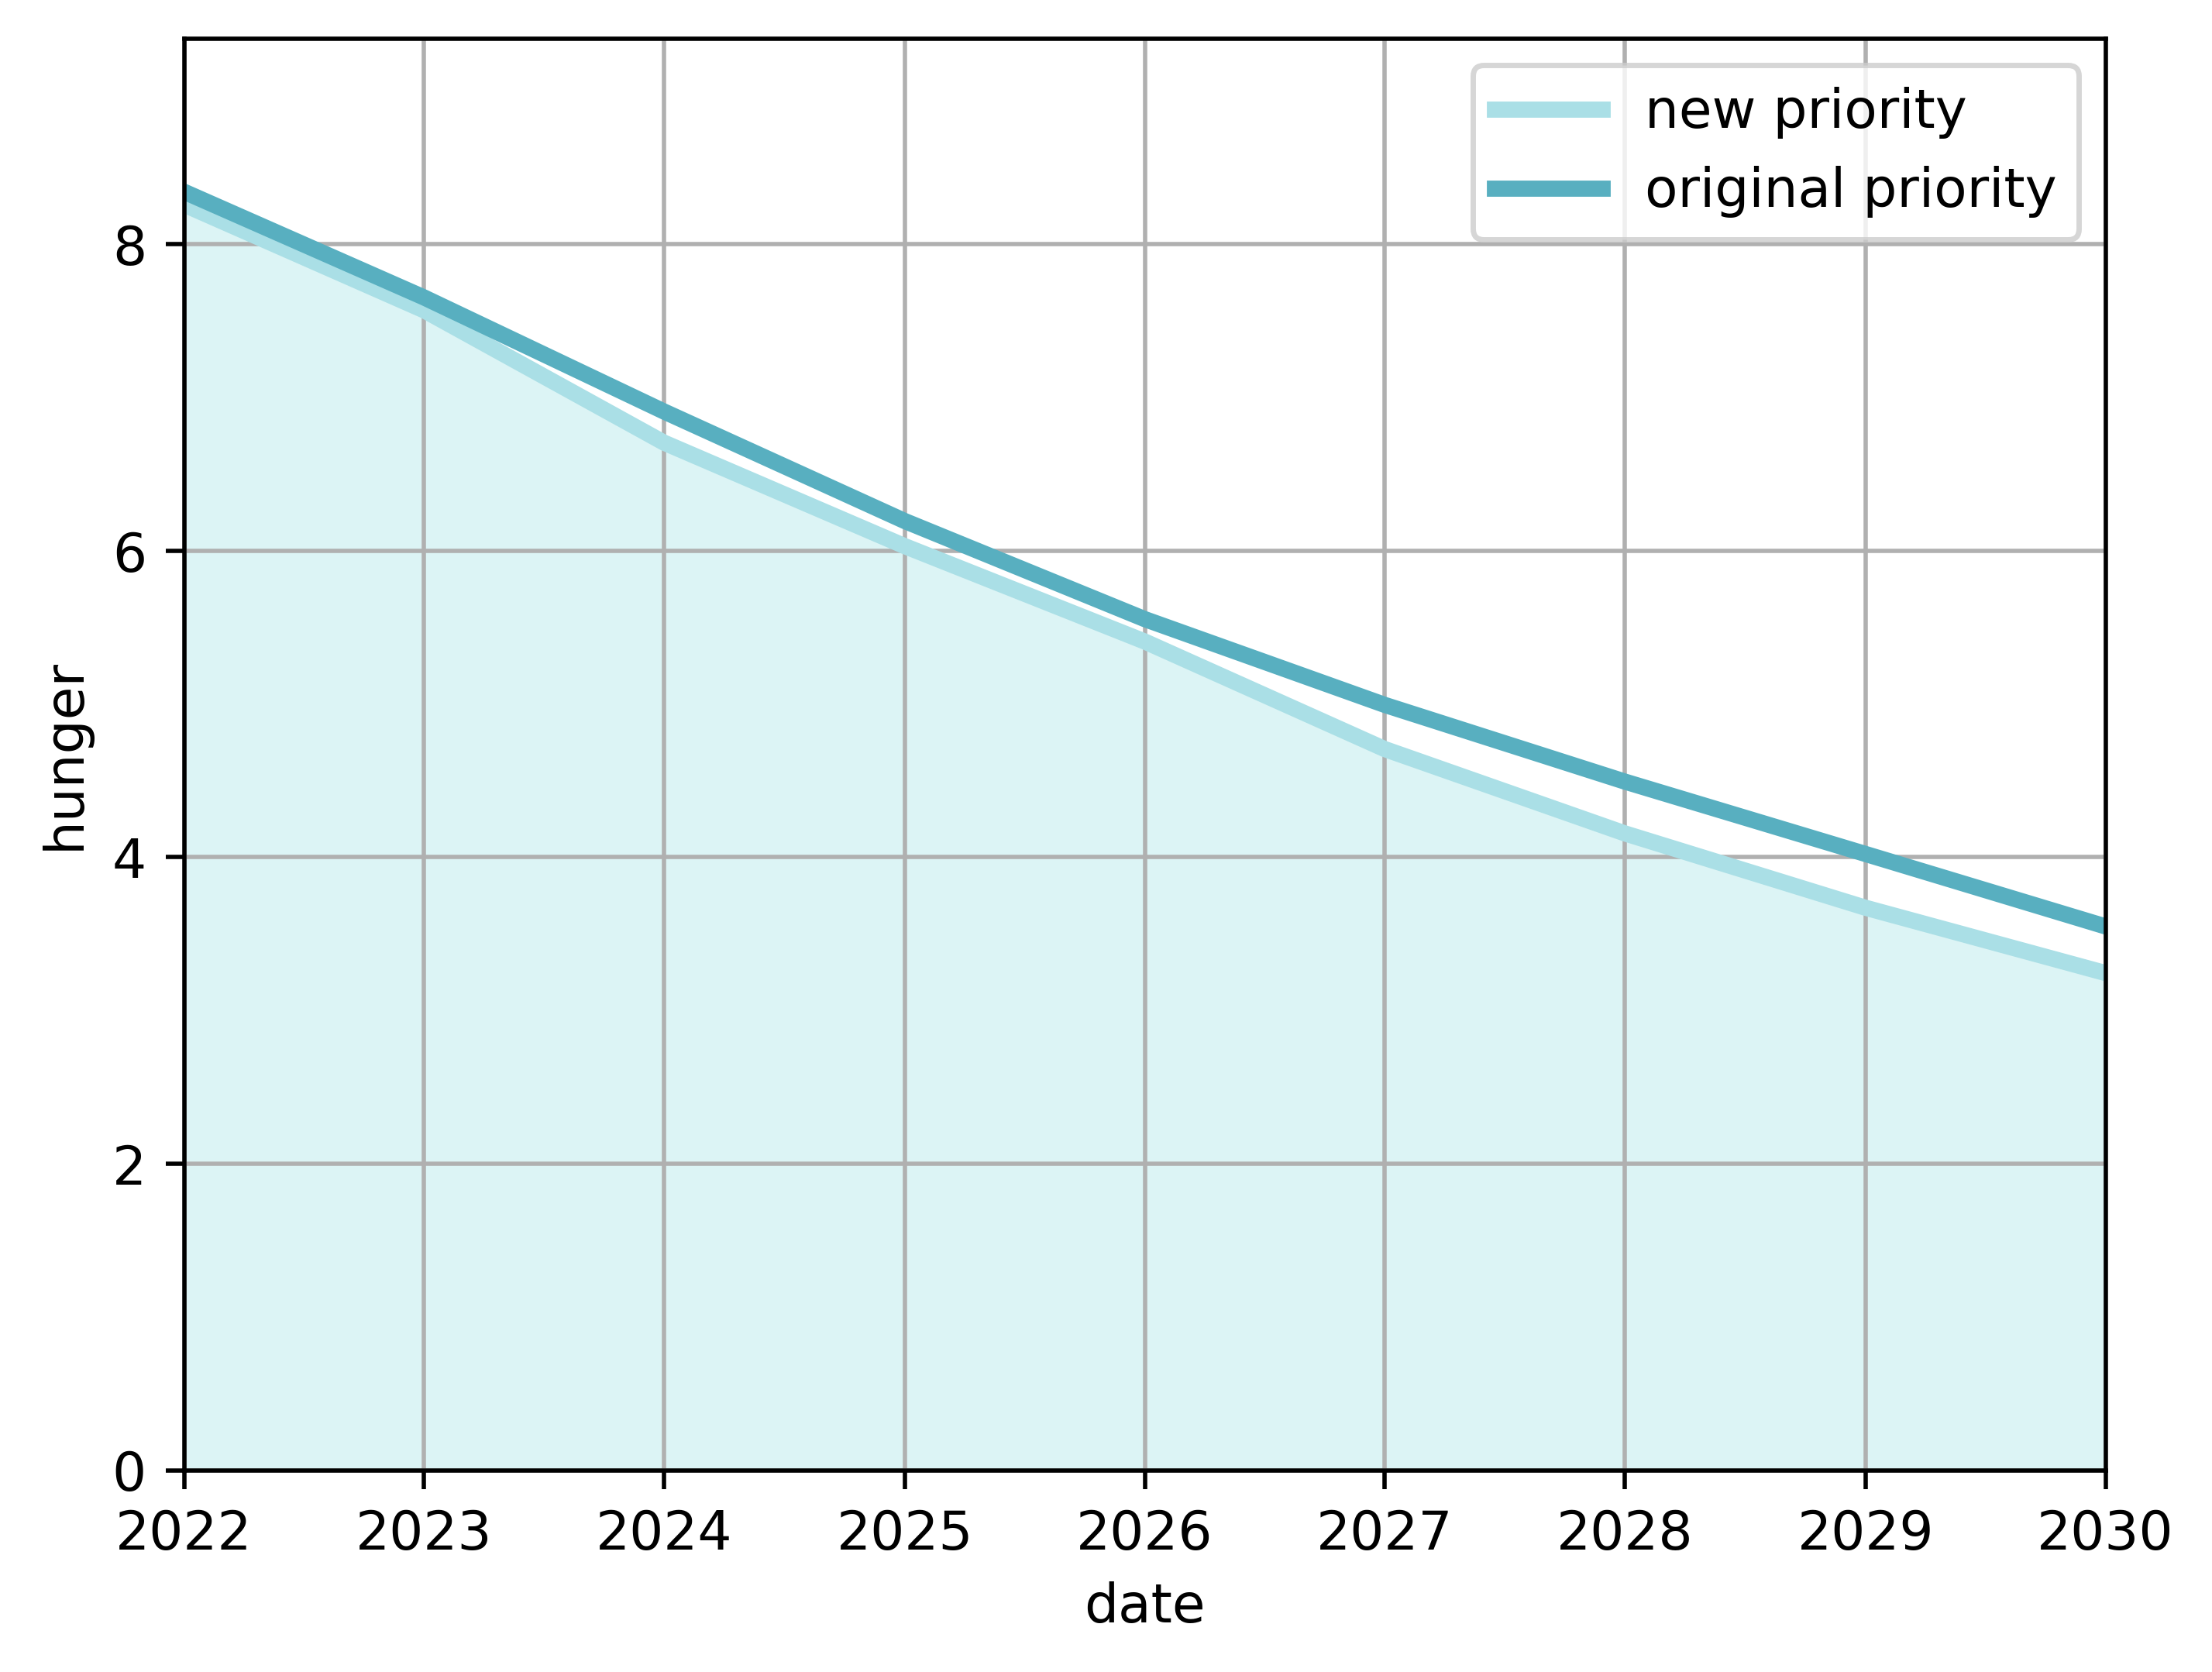
\includegraphics[height=6cm]{hunger.png}
       \caption{Comparison between two systems.}
        \label{fig:hunger}
       \end{minipage}
\end{figure}

Then we apply our SEPEG model to make a prediction of the Hunger Index, and the comparison of two systems is shown in Figure \ref{fig:hunger}. \textbf{Apparently, our model put more emphasis on the food equity, so $HI$ drops more steeply than the current food system.} However, the curve still has a distance from the point of 2.5. Achieving Zero Hunger is still difficult in our SEPEG system before 2030.

\subsection{Prediction of Food Insecurity Index by GM}
Food Insecurity, defined as the proportion of the population facing moderate or severe difficulties in accessing food, is also an significant indicator when describing the degree of hunger \cite{fii}.

To make a forecast for the Food Insecurity Index in 2030. We apply \textbf{Grey Forecast Model (GM)} to fit the situation. Based on only a small amount of information, Grey Forecast Model first carry out the correlation analysis, and the original data is generated and processed to find the law of system change. We then establish the corresponding differential equation, to predict the situation of the future development trend.

Considering the feature of the Food Insecurity Index, we adopt \textbf{GM (1,1) }in this problem. We first obtain the \textbf{accumulating generate operator}, $X^{(1)}=(\sum_1^1{x^{(0)}}, \sum_1^2{x^{(0)}} \dots \sum_1^n{x^{(0)}}  )$, where $x^{(0)}$ is the original data. Then we calculate the \textbf{mean generation sequence}  ${z^{(1)}(i)}= \frac{1}{2}({x^{(1)}(i-1)}+{x^{(1)}(i)})$, where ${x^{(1)}(j)}$ is the element of $X^{(1)}$. Therefore the equation of one order single variable grey model is carried out.

\begin{equation}
\label{Eq:GM}
{x^{(1)}(i)}+a{z^{(1)}(i)}=b,\quad \text{where}\quad i=1, 2 \dots n
\end{equation}

By least square method, we work out the answer, which is shown in Figure \ref{fig:gray}. In general, the trend of the Food Insecurity Index is downward, which depicts a bright future for us. Through the comparison in Figure \ref{fig:FII}, we can see that \textbf{the results of the SEPEG model is still better than the current food system due to its emphasis on the food equity.}

\begin{figure}[H]
    \begin{minipage}[c]{0.5\textwidth}
       \centering
       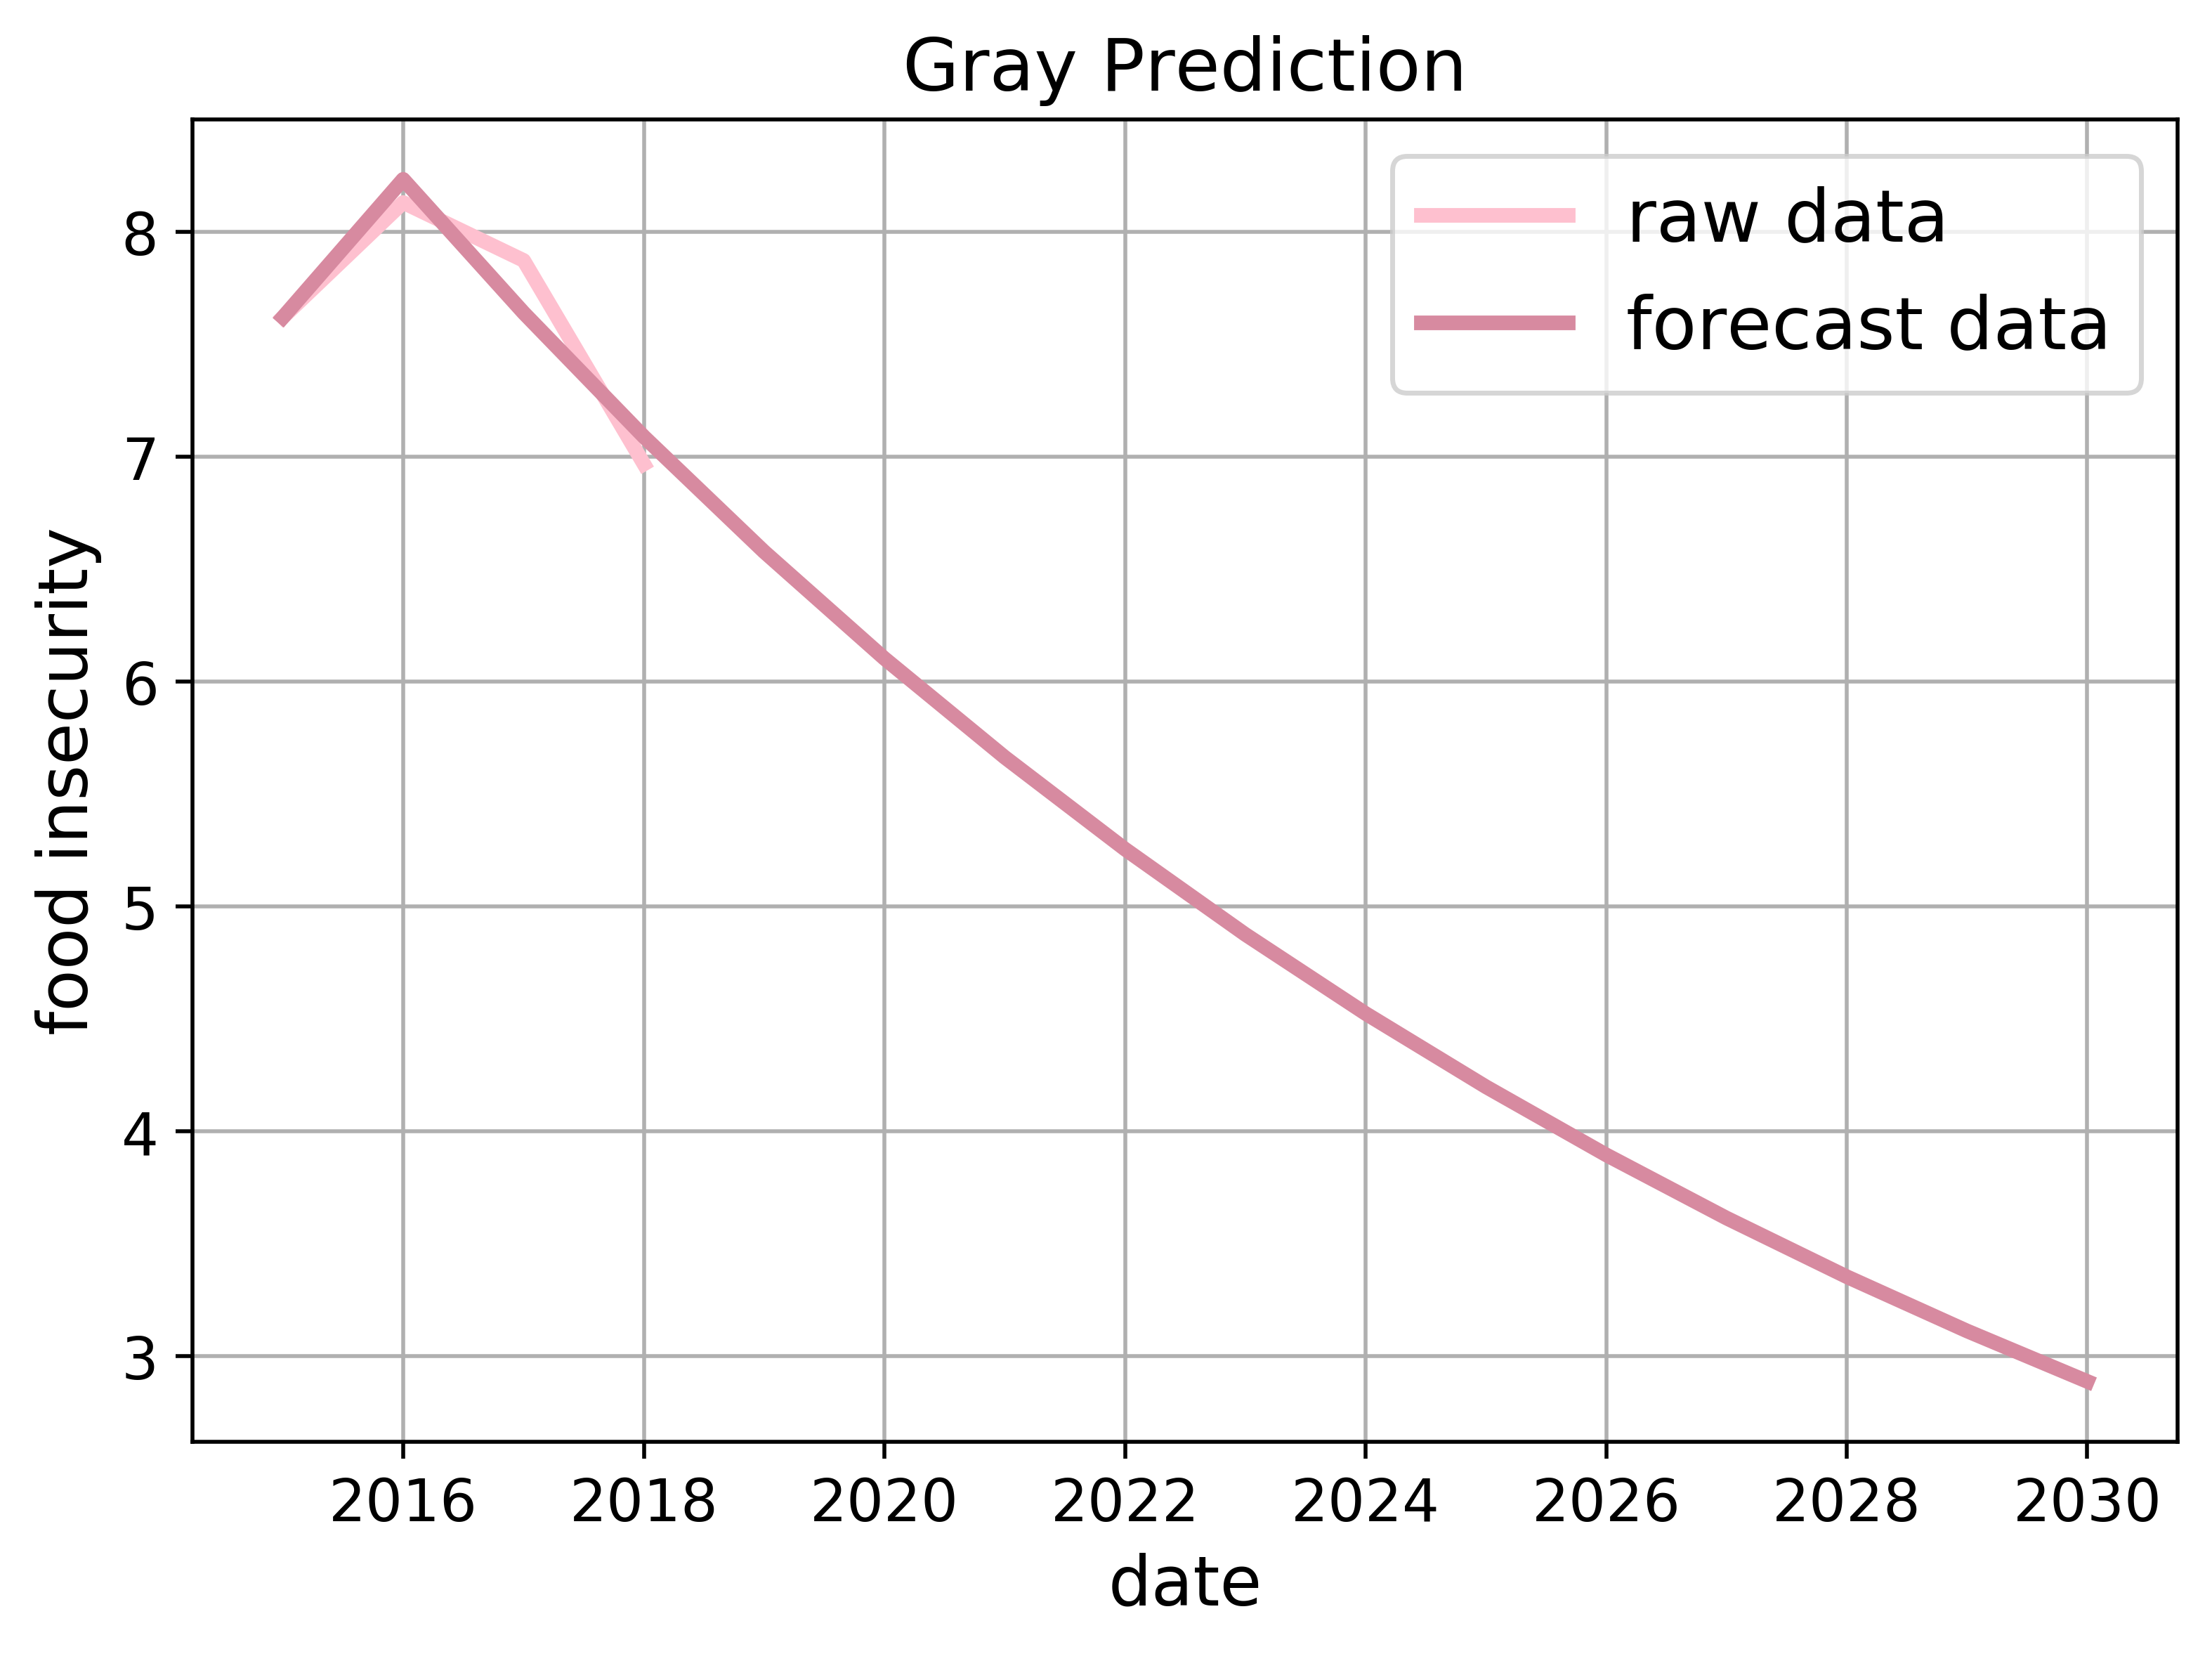
\includegraphics[height=6.2cm]{gray.png}
       \caption{Prediction of $FII$ by GM.}
       \label{fig:gray}
       \end{minipage}
    \begin{minipage}[c]{0.5\textwidth}
       \centering
       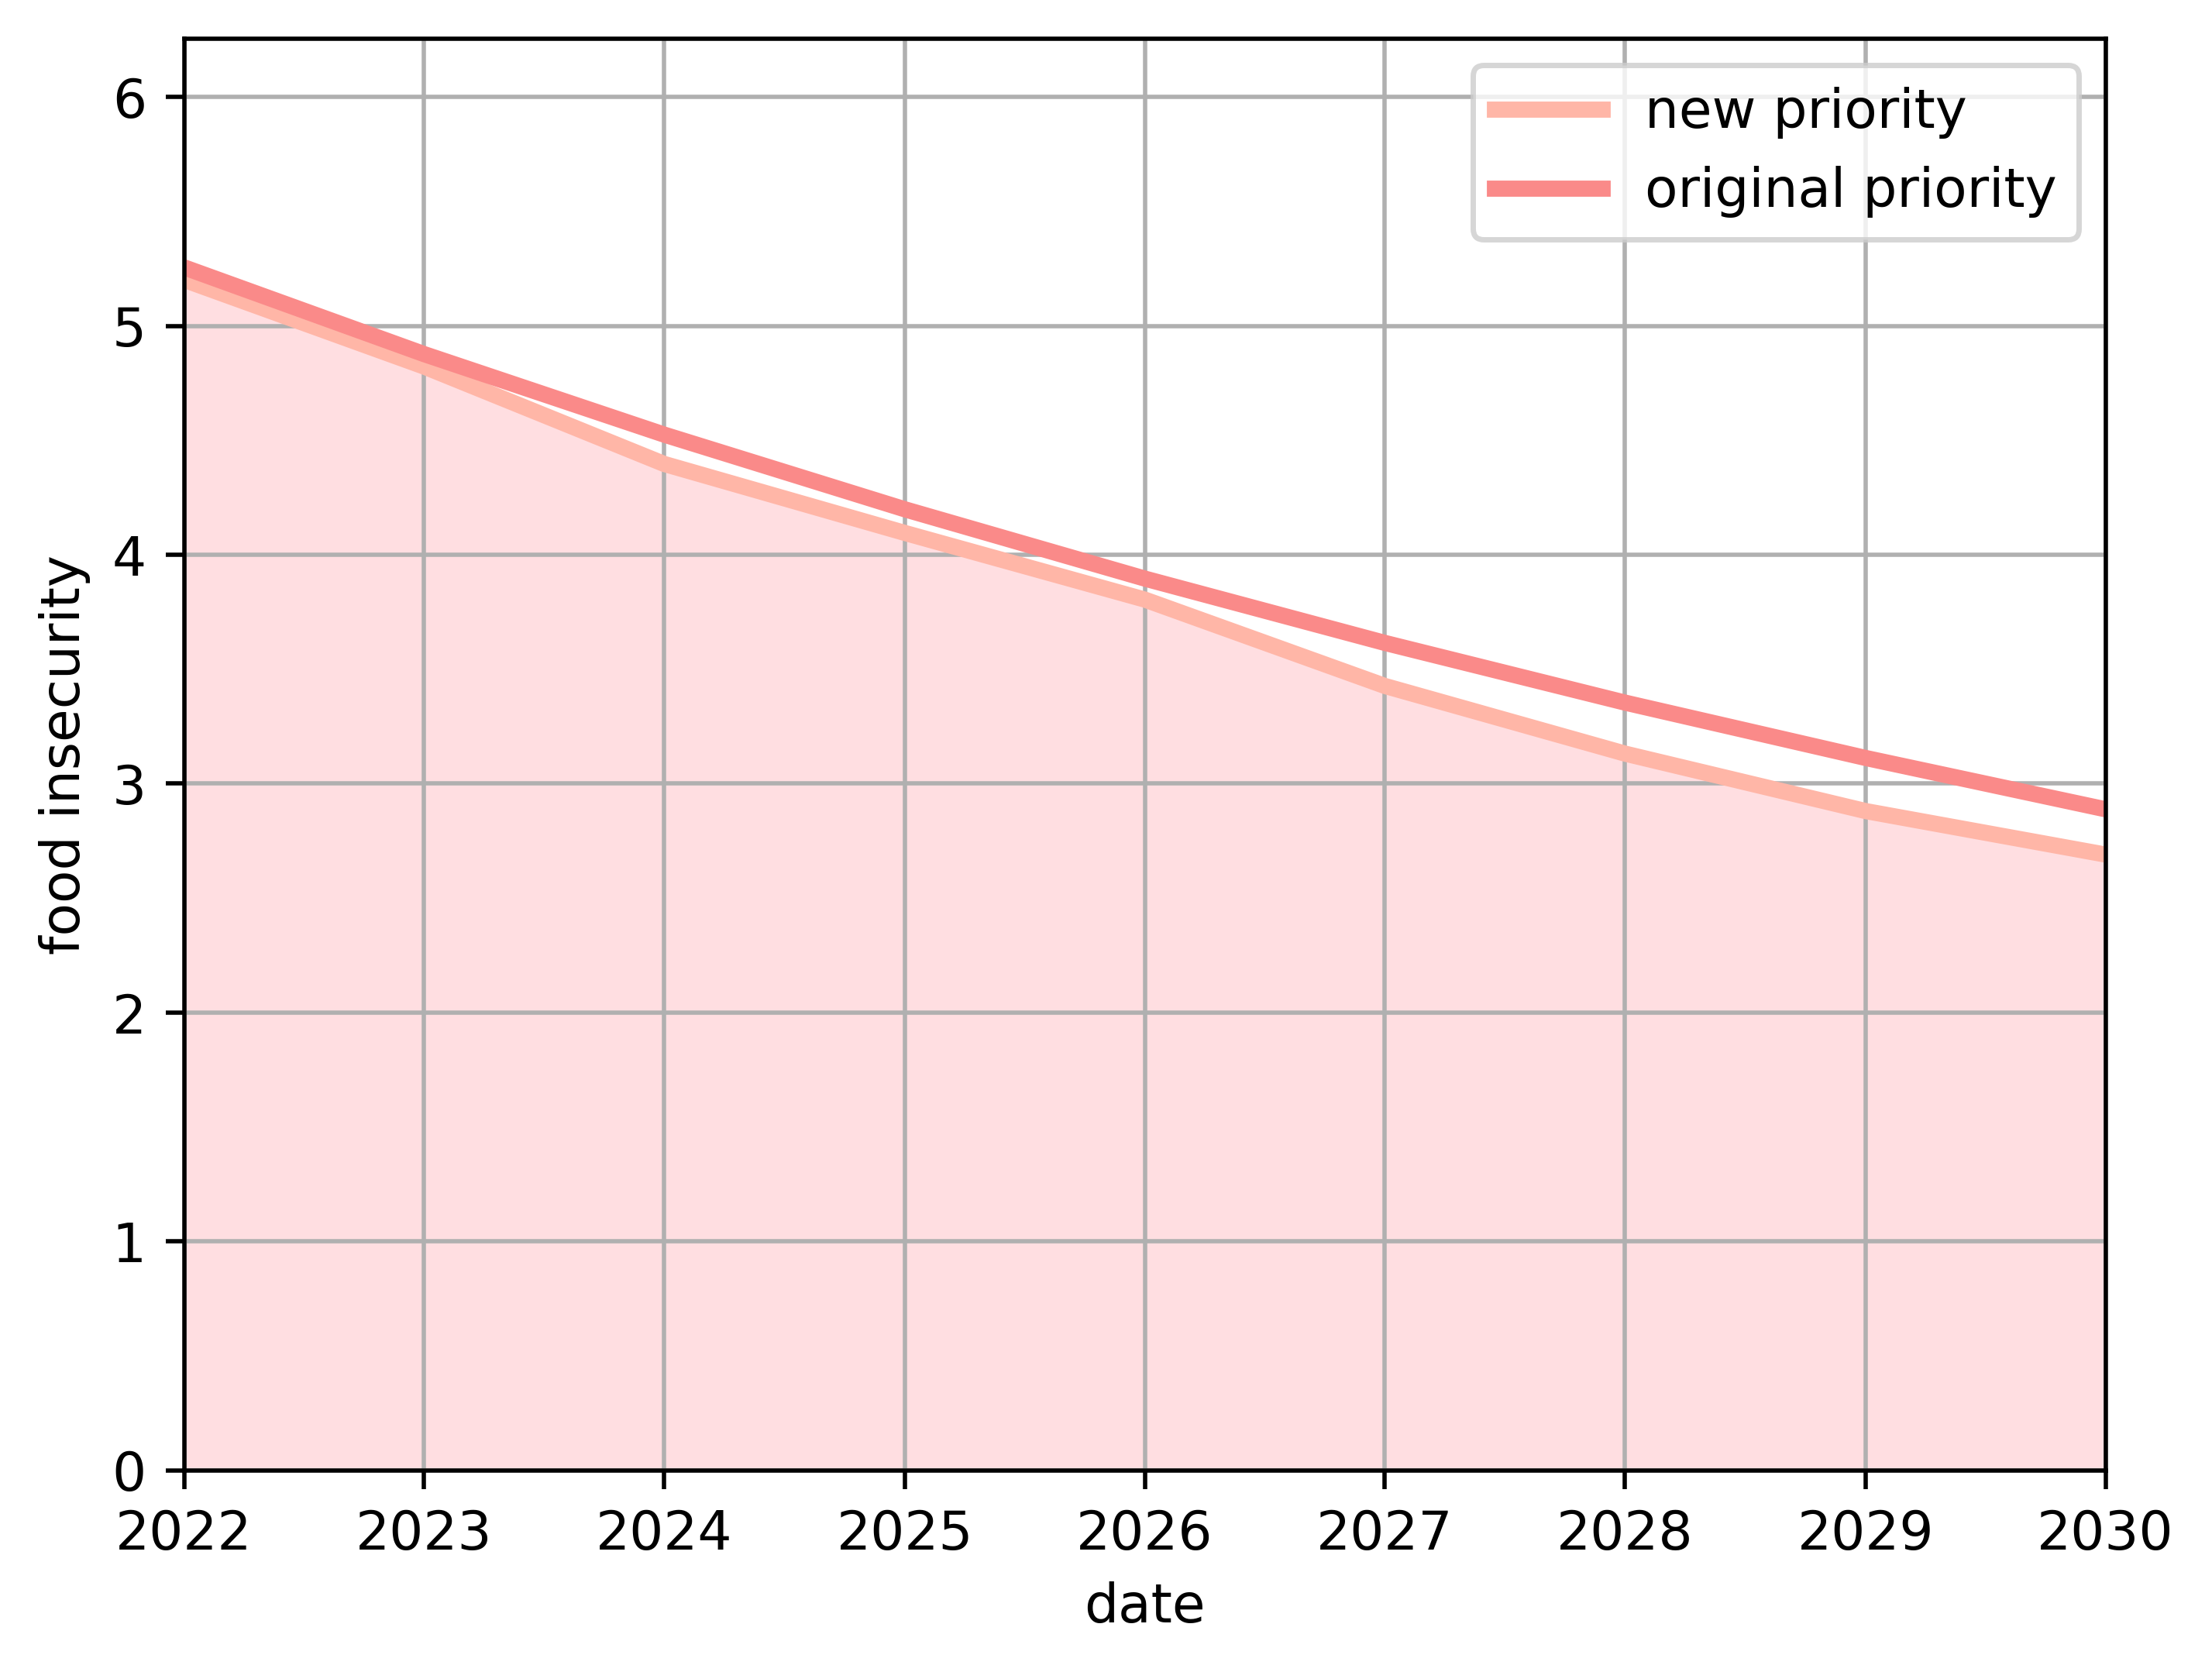
\includegraphics[height=6.2cm]{unsafe.png}
       \caption{Comparison between two systems.}
        \label{fig:FII}
       \end{minipage}
\end{figure}

 

From the predictions made above, we can see from a mathematical point of view that Zero Hunger\textbf{ can not be achieved by 2030}, which is also very much in line with the actual international situation. Regional conflict, climate change and extreme events are already becoming inevitable factors preventing us from ending hunger. What's worse, COVID-19 pandemic and the unprecedented desert locust epidemic in East Africa have made the global economic outlook uncertain, so the situation is even more severe\cite{pdf}.\textbf{ Zero Hunger still remains a goal that all mankind must spare no effort to strive for.}



\section{Scalability And Adaptability}

Scalability and adaptability are the two key indicators to measure the practicability and reliability of a model. The higher the values are, the wider our model's application range is. High scalability and adaptability can better satisfy the demands of countries and international organizations to upgrade the existing food system. Therefore, the system based on the new model is convenient for users to operate and maintain in future deployment. In this part, we choose two another cases, one is \textbf{Asia(part)} and the other is \textbf{South Korea} to check SEPES Model's performance.

\subsection{Scalability Verification}
\label{Sec-SV}
To verify the scalability, we decide to select the validation object from a larger scale. Asia, especially the east and southeast Asia, encompasses many developed and developing countries, including some of the world's main leading economies while people of some other countries are still struggling for a living below the poverty line. Therefore, we select this area, which can be regarded as the region requiring to implement the concept of sustainable development and social equity most in some degree to some extent.

As the overall data of the whole region is difficult to obtain from open channels, we integrate the data of individual country belonging to this area. Meanwhile, considering that countries with a population less than 10 million have little impact on the whole region, we abandon them during analysis. There are 11 countries altogether and we label this whole area as \textbf{Asia(part)}.

Then, following the previous steps, we use our model to forecast  indexes in the coming decade. Compared with the conclusions summarized in Section \ref{sec-App}, we find that changes of various indexes are in line with our expectations, as \textbf{regional sustainability and social equity are remarkably improved. What calls for attention is that the changing trend is very similar to the developing country's. }For example, in Figure \ref{fig:cool}, $WRI$ of Asia(part) and Indonesia are quite close, we think that the majority of this region are developing countries can explain this phenomenon.

\begin{figure}[H]
	\centering
	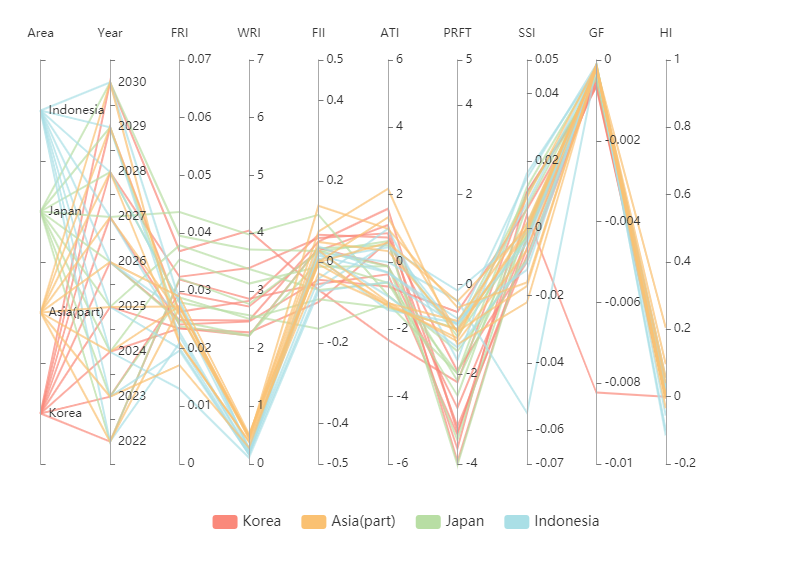
\includegraphics[height=10.5cm]{echarts (12).png} 
	\caption{Changing trends of indexes in different regions.}
	\label{fig:cool}
\end{figure}

\subsection{Adaptability Research}

Adaptability is another significant criterion to judge the quality of the model. Here, we select South Korea for further research. Based on the data of the Republic of Korea arranged before, we apply our model to it and the corresponding process is similar to that in Section \ref{Sec-SV}. 

In all, changes in eight indexes of South Korea conform to the optimization goal. \textbf{As a developed and prosperous nation in Asia, these changes share more similarities to Japan which is also one developed nation compared with Indonesia.} These similarities not only reflect the adaptability of our SEPES Model, namely the broad sphere of application, but further give a convincing demonstration of our model's accuracy. The specific changing trends of the indexes combined with previous regions are vividly visualized in Figure \ref{fig:cool} altogether. 

In sum, through detailed scalability verification and rigorous adaptability research, the SEPES Model \textbf{shows its outstanding ability in adapting to different places and scales, thus greatly proving the operability and practicability of our model. 
}
\section{Sensitivity Analysis}
To test the robustness of the SEPEG Model, we conduct sensitivity analysis on the customization parameters $RID1$ and $RID2$ in Equation \eqref{eq RID}, which depict the degree of the resource inclination. We alter $RID1$'s value from $0.01$ to $0.1$ and the value of $RID2$ is changed from $0.001$ to $0.01$. The corresponding change of Water Resource Index ($WRI$) is displayed in Figure \ref{fig:SA}.

\begin{figure}[H]
	\centering
	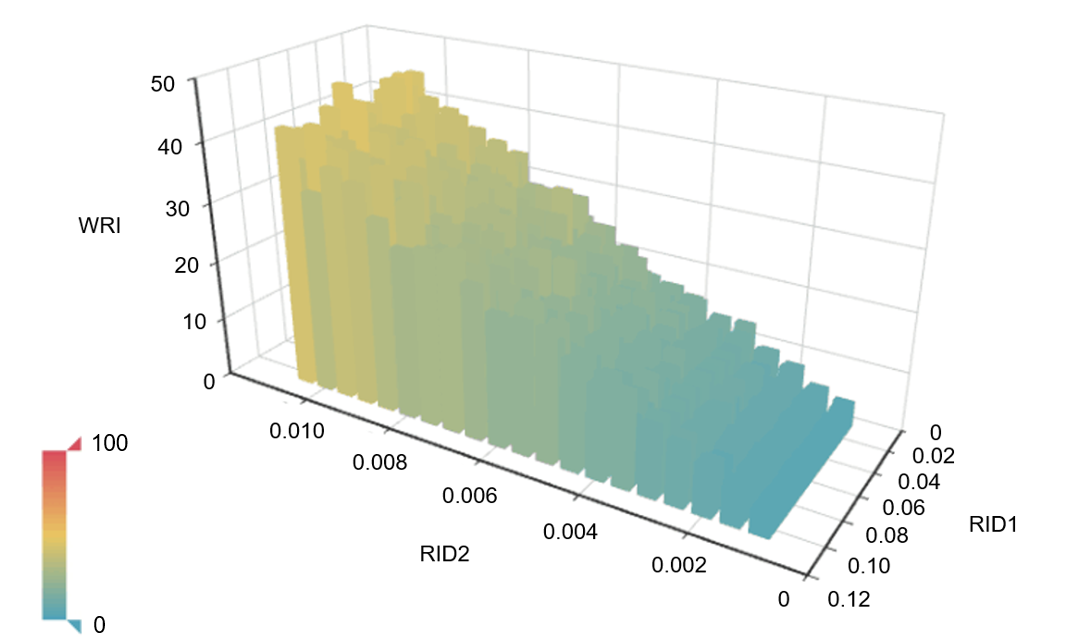
\includegraphics[height=8.5cm]{SA.png} 
	\caption{Influence of $RID1$ and $RID2$.}
	\label{fig:SA}
\end{figure}

\textbf{By observing Figure \ref{fig:SA}, we notice that the $WRI$'s tendency has little correlation with $RID1$ while it varies sharply when $RID2$ changes.} Considering that Average Daily Change ($\delta_d$) usually varies little day by day while the annual index value itself is relatively quite large, it's understandable that $RID2$ which functions on the annual index value is the sensitive parameter while $WRI$ is insensitive to $RID1$. Therefore, before applying the SEPES Model, we need to modify $RID2$' value carefully according to different situations. Generally speaking, our model shows the characteristic of stability to some degree.

\section{Strengths And Weaknesses}
\textbf{Strength}
\begin{itemize}
    \item The combination of subjectivity and objectivity is one major highlight of SEPEG Model. In the process of weighing different indicators, we preliminarily determine them based on the current data mining and further amend them subjectively in the pursuit of the optimized goal, which ensures the accuracy and validity of our model.
    
    \item The selection and quantification of the global factor is creative and pioneering. Considering that foreign trade surplus generally reflects a country's position in the global production chain, we pay more attention to export trade. Meanwhile, COVID-19 event has cast a shadow over economic globalization and the impact will continue for a long time. We also take this factor into account, making our model more practical and timely.
    
    \item The method we choose to simulate changes of indexes is very ingenious. By the aid of Roulette Wheel Selection, we can simulate the transition direction of the world more authentically and forecast the future changes more in line with the reality.
    
    \item Extensibility and clarity are also SEPEG Model's sharp edges, as we take into account most major factors that can affect food systems during modeling. For most food systems, we can get results in accord with the optimized goal and the results coincide with different national conditions and different economic development stages very well after applying the SEPEG Model.
    \item Our estimates of implementation time are pioneering,  as we quantify the costs of profitability in the new system and obtain an inequality. Based on the inequality, forecasts of implementation time will become stylized.
    \item Equity and sustainability are the most important aspects of the optimized food system, which is worthy of  most of our consideration. SEPEG model has three indicators to quantify them, covering many areas such as environment, food waste and hunger. Therefore our model can lay emphasis on sustainability and equity in a more comprehensive way.
    
\end{itemize}
\textbf{Weakness}
\begin{itemize}
     \item Due to the difficulty to obtain relevant data, our model dismisses the differences of statuses between developed and developing countries in international trade.
     
     \item During the establishment of the model, we attempt to select indexes with low correlation as far as possible and they are assumed to be independent in subsequent calculations, which may cause deviation in future prediction.
     
     \item The Resource Inclination Index ($RID$) is set and modified by our team according to intuitive experience and relevant domestic data. Actually, the value may vary of different times due to related domestic policy and strategies.
    
\end{itemize}





\newpage


%\bibliographystyle{IEEETran}
\bibliographystyle{ieeetr}
\bibliography{newrefs}

\newpage

\begin{appendices}
\paragraph{Appendix A \quad Tables\\[6pt]}

\quad \quad \quad \quad \quad \quad \quad Table 5: The annual variation of 8 indexes in Indonesia                  
\begin{figure}[H]
    \centering
    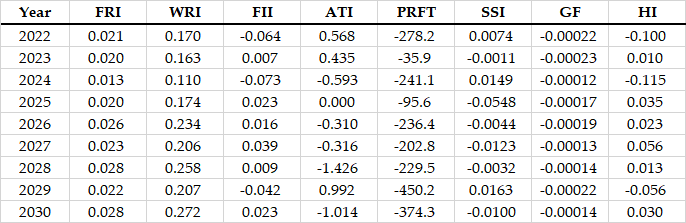
\includegraphics[width=16cm]{indonesia.png}
\end{figure}

\quad \quad \quad \quad \quad \quad \quad \quad Table 6: The annual variation of 8 indexes in Japan                  
\begin{figure}[H]
    \centering
    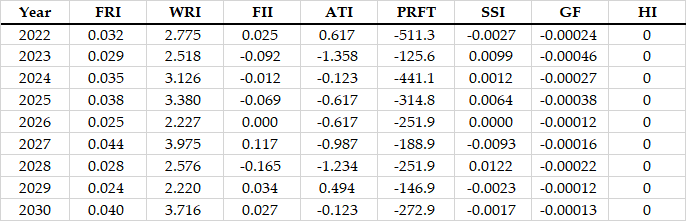
\includegraphics[width=16cm]{japan.png}
\end{figure}

\quad \quad \quad \quad \quad \quad \quad \quad Table 7: The annual variation of 8 indexes in Korea                  
\begin{figure}[H]
    \centering
    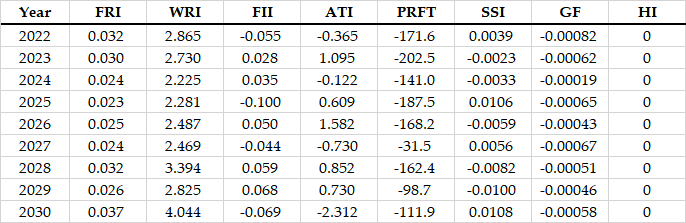
\includegraphics[width=16cm]{korea.png}
\end{figure}



\paragraph{Appendix B \quad Main Code\\[6pt]}


\lstinputlisting[language=Python]{2.py}
\end{appendices}



\end{document}


